
\documentclass [12pt,letterpaper]{exam}
\usepackage{amsmath, amsthm, amsfonts, amssymb, amscd}
\usepackage{type1cm}
\usepackage{amsmath}
\usepackage{amssymb}
\usepackage{amsthm}
\usepackage{latexsym}
\usepackage{amsfonts}
\usepackage{listings}
\usepackage{graphicx}
\usepackage{subcaption}
\usepackage{algorithm}
\usepackage{algorithm2e}
\newcommand{\R}{\mathbb{R}}
\newcommand{\comment}[1]{}
\newtheorem{theorem}{Theorem}
\newtheorem{lemma}{Lemma}[section]
\newtheorem{remark}{Remark}[section]
\newtheorem{corollary}{Corollary}[section]
\newtheorem{proposition}{Proposition}[section]
\newtheorem{conjecture}{Conjecture}[section]
\newtheorem{example}{Example}[section]
\newtheorem{definition}{Definition}[section]
\newcommand{\eop}{\hfill $\sqcap\!\!\!\!\sqcup$} % end of proof
%
\def\be{\begin{equation}}
\def\ee{\end{equation}}
\def\bea{\begin{eqnarray}}
\def\eea{\end{eqnarray}}
\def\proofbox{\blacksquare}
\def\bydef{\stackrel{\Delta}{=}}
\newcommand{\reals}{{\mathbb R}}
\newcommand{\natnums}{{\mathbb N}}
\newcommand{\naturals}{\mathds{N}}
%\usepackage{graphicx}

%\pagestyle{plain}

\oddsidemargin  0.0in
\evensidemargin 0.0in
\textwidth      6.0in
\headheight     0.0in
\topmargin      0.0in
\textheight     9.0in

\header{ECSE-507}{Optimization and Optimal Control}{18 March 2022}

\newcounter{count}

%%%%%%%%%%%%%%%%%%%%%%%%%%%%%%%%%%%%%%%%%%%%%%%%%%%%%%%%%%%%%%%%%%%%%%%%%%%%%%%%%%%%%%%%%%%%%%%%%%%%

\begin{document}
\vspace*{5mm}
\begin{center}
{\LARGE\bf McGill University }\\[5mm]
{\LARGE\bf Course ECSE-507 semester 2022 }\\[3mm]
{\LARGE\bf Optimization and Optimal Control}\\[5mm]
\end{center}

\flushleft{
\begin{tabbing}
XXXXXXXXXXXXXXXXXXXXXXX\= XXXXXXXXXXXXXXXXXXXXXXXX\= \kill
 {\bf Instructor} \\[1mm]
Hannah Michalska   \\[4mm]
\\\end{tabbing}
\begin{center}
\LARGE\bf{PROJECT REPORT}
\end{center}
\flushleft{
{\large\bf AUTHORS:}
\begin{tabbing}
XXXXXXXXXXXXXXXXXXXXXXX\= XXXXXXXXXXXXXXXXXXXXXXXX\= \kill
{\bf Banuso Abdulquadri Oluwatobi} \> {\bf Amal Koodoruth} \\
{\bf 260669341 } \> {\bf 260831147}\\[5mm]
\\\end{tabbing}
{\Large\bf Personal Declaration}\\[3mm]
{\large\it We wish to state that the work presented here has been carried out by the authors alone. No part of it has been copied from the internet or other sources, unless clearly acknowledged, and no part of it has been shared with other students.}\\[3mm]
\flushleft{
\begin{tabbing}
XXXXXXXXXXXXXXXXXXXXXXX\= XXXXXXXXXXXXXXXXXXXXXXXX\= \kill
{\bf Banuso Abdulquadri Oluwatobi } \> {\bf Amal Koodoruth} \\[7mm]
{Abdulquadri} \> {Amal}\\
{260669341} \> {260831147}\\
\\\end{tabbing}
}

\clearpage

\clearpage
\section{Unconstrained Optimization}
The code solving the unconstrained optimization problems can be found in the software package submitted.
There are different search algorithms used to find the solutions to unconstrained nonlinear problems briefly explained below. 
\textbf{\subsection{Algorithms To Solve Unconstrained Nonlinear Programming Problems}} 
There are different algorithms that can solve general unconstrained nonlinear programming problems. These include:
\begin{enumerate}
    \item Steepest Descent search algorithm
    \item Secant Algorithm
    \item Conjugate gradient Method
\end{enumerate}
\subsubsection{Steepest Descent Algorithm}
 Steepest Descent is a first-order iterative optimization algorithm to find a local minimum of a differentiable function. The idea is to take repeated steps in the opposite direction of the gradient of the function at the current point, because this is the direction of steepest descent. Overview of the Steepest Descent Algorithm is provided below: 
\SetKwInOut{Input}{Input}
\SetKwInOut{Output}{Output\,}
\SetAlgoLined
\DontPrintSemicolon
\begin{algorithm}[H]
   \textbf{Choose $x_{0}$ \in \mathbb{R}^{n}. Set\hspace{2mm}i = 0}: \newline
   \textbf{Iteration j: } \\
   (1) : Stop \hspace{2mm} if \hspace{2mm} $\nabla V (x_{j})$ = 0 as then $x_{j}$ satisfies a necessary condition for a local minimizer. \\
   (2) : Set $s_{j}$ := -$\nabla V(x_{j})$ \\
   (3) : Choose a scalar $\omega_{j} > 0$, so $V(x_{j} + \omega_{j}s_{j})$ is less than $V(x_{j})$, typically $\omega_{j}$ is chosen to minimize $V(x_{j} + \omega s_{j})$ with $\omega \in \mathbb{R}$\\
   (4) : Set j = j+1 and return to first step.\\
  \caption{\textsc{Steepest Descent Algorithm}}
\end{algorithm}
\subsubsection{Secant Algorithm}
The secant method is a root-finding algorithm that uses a succession of roots of secant lines to better approximate a root of a function f. The secant method is a finite-difference approximation of Newton's method. It is also known as a quasi-newton method. Overview of the Secant Algorithm is provided below: 
\SetKwInOut{Input}{Input}
\SetKwInOut{Output}{Output\,}
\SetAlgoLined
\DontPrintSemicolon
\begin{algorithm}[H]
   \textbf{Choose $x_{0}$ \in \mathbb{R}^{n}.}: \newline
   \textbf{Symmetric positive definite $H_{0} \in \mathbb{R}^{n x n}$, $H_{0}$ is an estimate of unknown $C^{-1}$}\newline 
   Set \hspace{2mm} j := 0 \\
   \textbf{Iteration} \hspace{2mm} j: \\
   (1) : Set \hspace{2mm} $s_{j}$ = -$H_{j}\nabla V(x_{j})$ (pseudo-Newton search direction). \\
   (2) : Choose $\omega_{j} \geq$ 0 so $V(x_{j} + \omega_{j}s_{j})$ less than $V(x_{j})$ \\
   (3) : Set $x_{j+1}$ = $x_{j} + \omega_{j}s_{j}$ \\
   (4) : Stop if $||\nabla V(x_{j+1})||$ less than $\epsilon$ = small \\
   (5) : $\triangle x_{j}$ = $x_{j+1} - x_{j}$, $\triangle g_{j}$ = $\nabla V(x_{j+1}) - \nabla V(x_{j})$ \\
   (6) : Choose symmetric positive definite $H_{j+1} \in \mathbb{R}^{nxn}$ so \\
   $H_{j+1} \cong C^{-1}$ - improved \\
   (7) : Set $j = j+1$ and return to (1) \\
  \caption{\textsc{Secant Algorithm}}
\end{algorithm}
The most famous way to choose $H_{j}$ is the David Fletcher Powell Algorithm. 

\subsubsection{Conjugate Gradient Method}
Conjugate direction methods can be regarded as being between the method of steepest descent (first-order method that uses gradient) and Newton’s method (second-order method that uses Hessian as well). It accelerates the convergence rate of steepest descent while avoiding the high computational cost of Newton’s method. Overview of the Conjugate Gradient Method is provided below:   
\SetKwInOut{Input}{Input}
\SetKwInOut{Output}{Output\,}
\SetAlgoLined
\DontPrintSemicolon
\begin{algorithm}[H]
   \textbf{Choose $x_{0}$ \in \mathbb{R}^{n}}: \newline
   Set\hspace{2mm} $s_{0}$ = -$\nabla V(x_{0}), j = 0$ \newline 
   (1) : Stop if $||V(x_{j})||$ is less than $\epsilon$ as then $x_{j} \cong x$ \\
   (2) : Choose $\omega_{j} \in$ arg min $V(x_{j} + \omega s_{j})$ \\
   $x_{j+1} = x_{j} + \omega_{j}s_{j}$\\
   (3) : Set $\beta_{j+1} = \frac{[\nabla V(x_{j+1}) - \nabla V(x_{j})]^{T}\nabla V(x_{j+1})}{||\nabla V(x_{j})||^{2}} \in \mathbb{R}$\\
   $s_{j+1} = \nabla V(x_{j+1}) + \beta_{j+1}s_{j}$\\
   the term $\beta_{j+1}s_{j}$ makes the conjugate gradient different from the steepest descent. \\
   $j = j + 1$ and return to (1) \\
  \caption{\textsc{Conjugate Gradient Method}}
\end{algorithm}

\subsection{Quadratic Optimization Problem}
The objective is to minimize the following cost function:
\begin{align}
& \mbox{(A)} : \ \ V(x) = 5+ \left[ \begin{array}{cccccc} 1 & 4 & 5 & 4 & 2 & 1 \end{array} \right] x + x^T \left[ \begin{array}{cccccc}  9 & 1 & 7 & 5 & 4 & 7 \\
1 & 11 & 4 & 2 & 7 & 5 \\ 7 & 4 & 13 & 5 & 0 & 7 \\ 5 & 2 & 5 & 17 & 1  & 9 \\
4 & 7 & 0 & 1 & 21 & 15 \\ 7 & 5 & 7 & 9 & 15 & 27 \end{array} \right] x ; \ \ x \in \mathbb{R}^6 \nonumber \\
\end{align}
This is an unconstrained quadratic optimization problem of the form:
\begin{align}
    V(x) = a + b^{T}x + \frac{1}{2}x^{T}Cx
\end{align},
where 
\begin{align}
    V \in \mathbb{R}, \hspace{2mm} a \in \mathbb{R}, \hspace{2mm} b \in \mathbb{R}^{n},\hspace{2mm} C \in \mathbb{R}^{nxn} \hspace{2mm} and \hspace{2mm} C^{T} = C  \hspace{2mm}& \hspace{2mm} C > 0
\end{align}
C is a positive definite symettric matrix.
This can be solved using the standard quadractic direct solution: 
\begin{align}
    x = -C^{-1}b
\end{align}
or using search algorithms: 
\begin{itemize}
    \item Steepest descent algorithms 
    \item Secant algorithms
    \item Conjugate gradient method 
\end{itemize}
\subsubsection{Solutions to Quadratic problem using our python programs and matlab benchmark \textit{quadprog} function: }
All 4 algorithms converged to the same minimal solution for $x$ with a tolerance set to be $tol =1e-8$ and the same initial value of all column vector of zeros. The gradient loss of the secant algorithm converged to a minimum fastest of our Python-implemented sub-programs as it requires one function evaluation per iteration, following the initial step and it does not require use of the derivative of the function $V(x)$,
while the steepest descent took longest to approach a minimum as it requires to constantly calculate the gradient derivative ($\nabla V(x)$) at every iteration step which is computationally expensive as can be seen in Figure 1. The matlab program used the algorithm \textit{ interior point convex} and quickly found a solution in 1 iteration. \newline All solutions correspond to the standard quadratic solution: 
\begin{align}
    x = -C^{-1}*b = \begin{bmatrix}
     0.3366 \\
    0.0560 \\
   -0.4300 \\
   -0.1920 \\
   -0.2713 \\ 
    0.2101 \\
    \end{bmatrix} 
\end{align}
\begin{table}[htbp]
\begin{center}
\begin{tabular}{|c|c|c|c|c|}
\hline
 & \textbf{Steepest Descent} & \textbf{Secant} &\textbf{Conjugate Method} &\textbf{\textit{quadprog}}\\
\hline
Iterations & 107 & 14 &37& 1 \\
\hline
$x$ & 
\begin{bmatrix}
0.3365 \\
 0.0560 \\
 -0.4300   \\
 -0.1919  \\
 -0.2713 \\
 0.2100 \\
\end{bmatrix}
&\begin{bmatrix}
 0.3365 \\
 0.05604  \\ 
 -0.4300 \\
 -0.1919 \\
 -0.2713 \\
 0.2100 \\
\end{bmatrix} & \begin{bmatrix}
0.3365 \\
0.05604\\
-0.4300 \\
-0.1919 \\
-0.2713 \\ 
0.2101\\
\end{bmatrix} &\begin{bmatrix}
     0.3366 \\
    0.0560 \\
   -0.4300 \\
   -0.1920 \\
   -0.2713 \\
    0.2101 \\
\end{bmatrix} \\
\hline 
\end{tabular}
\label{table:results}
\caption{Algorithm Performance}
\end{center}
\end{table}

\begin{figure}[h!]
\begin{subfigure}[t]{0.6\textwidth}
\centering
    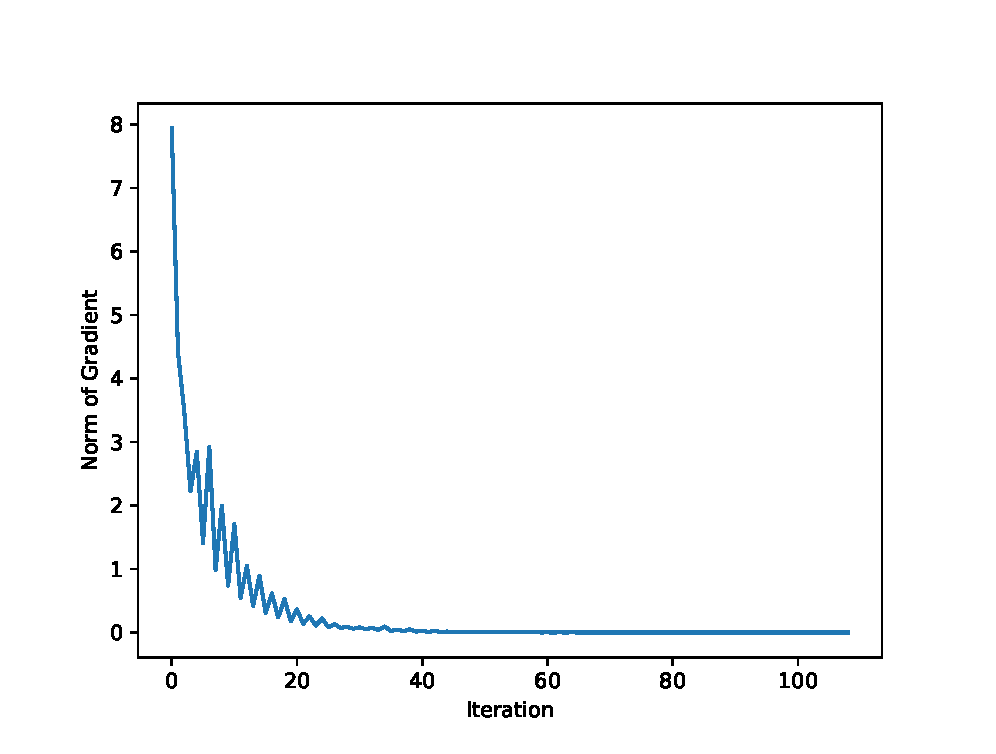
\includegraphics[width=\textwidth]{images/python/sd-pA.eps}
\caption{}
\end{subfigure}
\hfill 
\begin{subfigure}[t]{0.6\textwidth}
\centering
    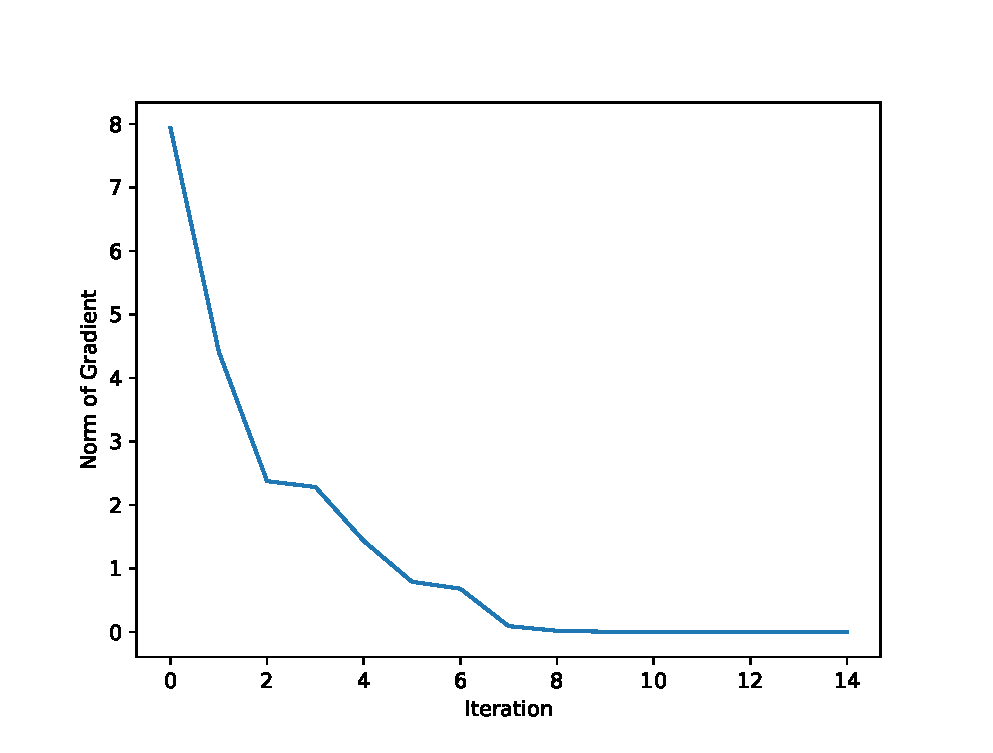
\includegraphics[width=\textwidth]{images/python/sec-pA.eps}
    \caption{}
\end{subfigure}
\hfill
\begin{subfigure}[t]{0.6\textwidth}
\centering
    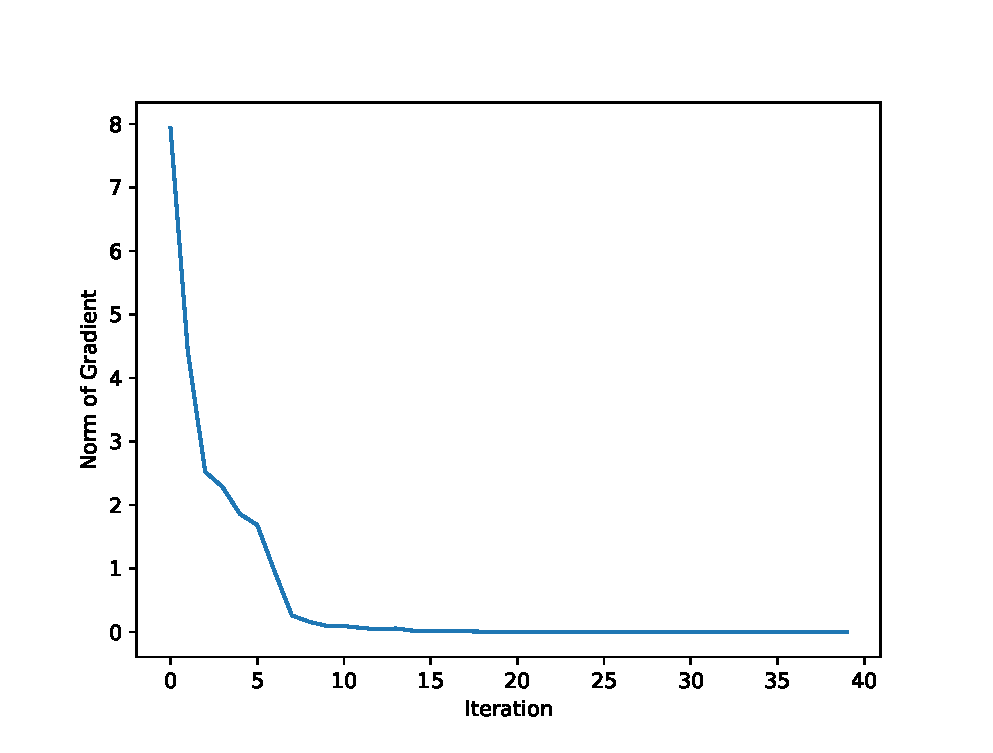
\includegraphics[width=\textwidth]{images/python/cg-pA.eps}
    \caption{}
\end{subfigure}
\caption{(a): Steepest descent, (b): Secant method, (c): Conjugate gradient}
\end{figure}
\clearpage
\subsection{Nonlinear Optimization problem}
The objective is to minimize the following cost function:
\begin{align}
\mbox{(B)} : \ \ V(x) = - \frac{\sqrt{(x_1^2 +1)(2x_2^2 + 1)}}{x_1^2 + x_2^2 + 0.5}; \ \  x \in \mathbb{R}^2 \nonumber \\
\end{align}
This is an unconstrained nonlinear optimization problem of the form:
\begin{align}
    V(x) = f(x)
\end{align}
where 
\begin{align}
    V \in \mathbb{R}
\end{align}
This can be solved using search algorithms: 
\begin{itemize}
    \item Steepest descent algorithms 
    \item Secant algorithms
    \item Conjugate gradient method 
\end{itemize}
\subsubsection{Solutions to unconstrained nonlinear problem using our python programs and matlab benchmark \textit{fminunc} function: }
All four algorithms converged to very close local minimal solutions for $x$ with a tolerance set to $tol =1e-8$ and the same initial value of the column vector of $[-1,1]^{T}$ as confirmed in the contour plot in figure 3. The gradient loss of the secant, conjugate and steepest descent algorithm of our Python-implemented sub-programs converged to a minimum at close to 6 iterations while the matlab implementation used the quasi newton method approached the minimum at 5 iterations.
The contour plot of the function $V(x)$ and the minimum solutions of $x$ derived from the 4 algorithms showed that the lowest value of the objective function for the 4 algorithms exists close to the local minima of the function.
\begin{table}[htbp]
\centering
\begin{center}
\begin{tabular}{|c|c|c|c|c|}
\hline
 & \textbf{Steepest Descent} & \textbf{Secant} &\textbf{Conjugate Method} &\textbf{\textit{Matlab}}\\
\hline
Iterations & 6 & 7 &7& 5 \\
\hline
$x$ & 
\begin{bmatrix}
-4.2345e-09 \\
-5.3553e-09 \\
\end{bmatrix}
&\begin{bmatrix}
 -2.8775e-09 \\
 -2.8274e-09 \\
\end{bmatrix} & \begin{bmatrix}
 -1.0739e-04 \\
 -6.8937e-05 \\
\end{bmatrix} &\begin{bmatrix}
   8.8494e-09 \\
    -2.6837e-10 \\  
\end{bmatrix} \\
\hline 
\end{tabular}
\label{table:results}
\caption{Algorithm Performance}
\end{center}
\end{table}

\begin{figure}[h!]
\centering
\begin{subfigure}[t]{0.4\textwidth}
\centering
    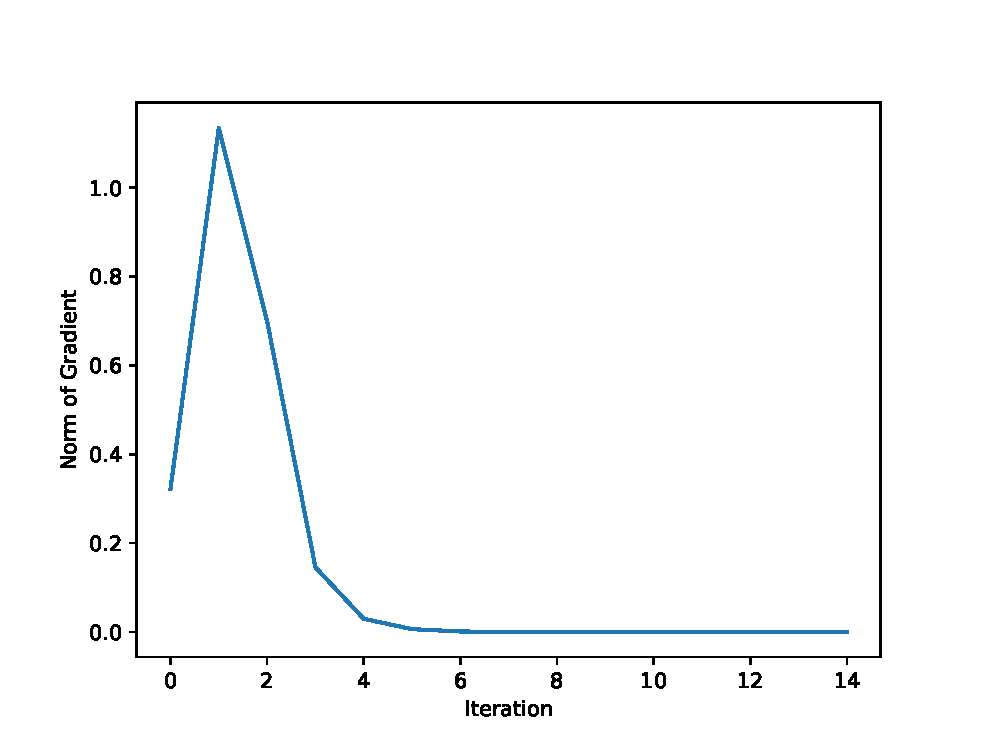
\includegraphics[width=\textwidth]{images/python/sd-pB.eps}
\caption{}
\label{fig:Class distribution}
\end{subfigure}
\hfill 
\begin{subfigure}[t]{0.4\textwidth}
\centering
    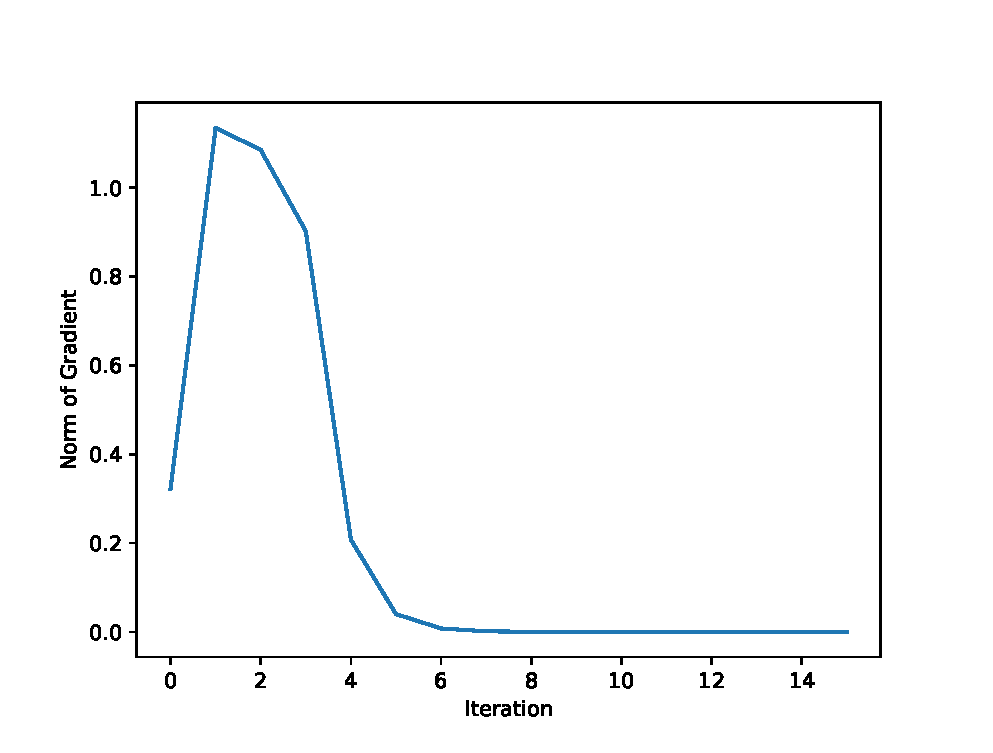
\includegraphics[width=\textwidth]{images/python/sec-pB.eps}
    \caption{}
    \label{fig:TSNE}
\end{subfigure}
\hfill
\begin{subfigure}[t]{0.4\textwidth}
\centering
    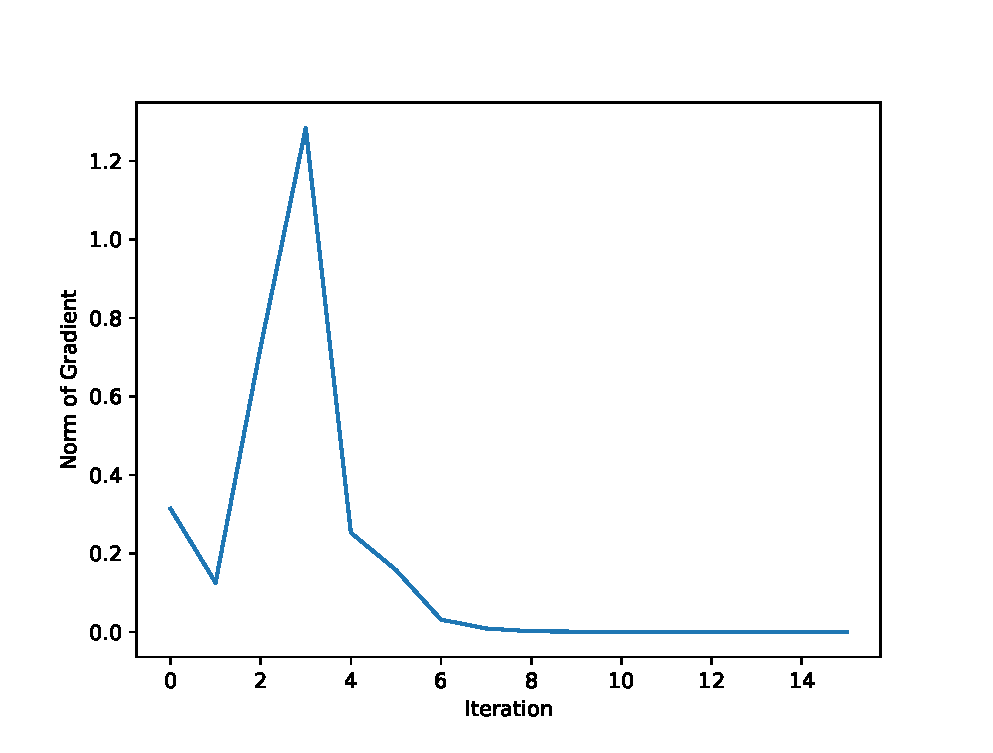
\includegraphics[width=\textwidth]{images/python/cg-pB.eps}
    \caption{}
    \label{fig:TSNE}
\end{subfigure}
\hfill
\begin{subfigure}[t]{0.4\textwidth}
\centering
    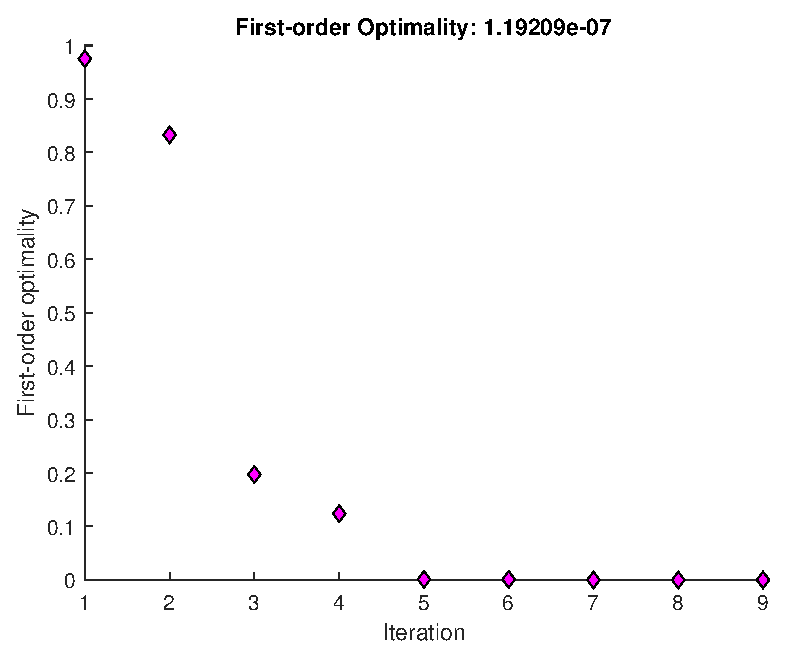
\includegraphics[width=\textwidth]{images/matlab/1b_loss.eps}
    \caption{}
    \label{fig:TSNE}
\end{subfigure}
\caption{(a): Steepest descent, (b): Secant method, (c): Conjugate gradient, (d): Matlab: \textit{fminunc - quasi-newton method}}
\end{figure}
\begin{figure}
    \centering
    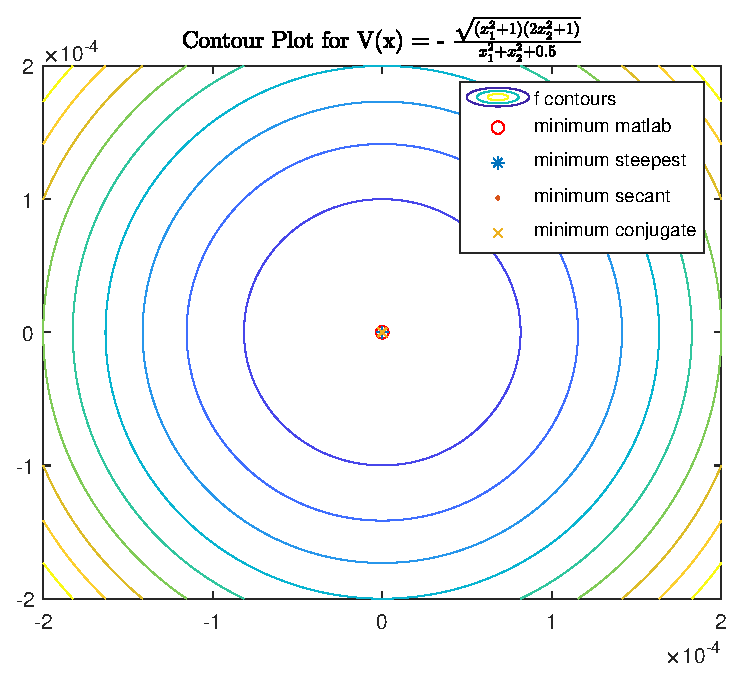
\includegraphics[width=0.4\textwidth]{images/matlab/matlab_1b.eps}
    \caption{Contour Plot for $V(x) = - \frac{\sqrt{(x_1^2 +1)(2x_2^2 + 1)}}{x_1^2 + x_2^2 + 0.5}$ }
\end{figure}
\clearpage
\subsection{Nonlinear Optimization problem}
The objective is to minimize the following cost function:
\begin{align}
& \mbox{(C)}: \ \  V(x) = 1 + \left[ \begin{array}{cc} 1 & 2 \end{array} \right] x + \frac{1}{2} x^T \left[ \begin{array}{cc} 12 & 3 \\ 3 & 10 \end{array} \right] x  \\
& \hspace{2cm} + 10 \mbox{ln}(1+ x_1^4) \mbox{sin}(100x_1)+ 10 \mbox{ln}(1+x_2^4) \mbox{cos}(100x_2)  ; \ \  x \in \mathbb{R}^2  \nonumber
\end{align}
This is an unconstrained nonlinear optimization problem of the form:
\begin{align}
    V(x) = f(x)
\end{align}
where 
\begin{align}
    V \in \mathbb{R}
\end{align}
This can be solved using search algorithms: 
\begin{itemize}
    \item Steepest descent algorithms: 
    \item Secant algorithms: 
    \item Conjugate gradient method: 
\end{itemize}
\subsubsection{Solutions to unconstrained nonlinear problem using our python programs and matlab benchmark \textit{fminunc} function: }
All 4 algorithms converged to very close local minimal solutions for $x$ with a tolerance set to $tol =1e-4$ and the same initial value of column vector of $[0,0]^{T}$ as confirmed in the contour plot in figure 5. The gradient loss of the secant and algorithm converged to a minimum fastest of our Python-implemented subprograms while the conjugate gradient took longest to approach a minimum as can be seen in Figure 4. The Matlab program used the \textit{quasi newton} algorithm and quickly found a solution in 5 iterations.
The contour plot of the function $V(x)$ and the minimum solutions of $x$ derived from the 4 algorithms showed that 
\begin{table}[htbp]
\centering
\begin{center}
\begin{tabular}{|c|c|c|c|c|}
\hline
 & \textbf{Steepest Descent} & \textbf{Secant} &\textbf{Conjugate Method} &\textbf{\textit{Matlab}}\\
\hline
Iterations & 7 & 7 &8& 4 \\
\hline
$x$ & 
\begin{bmatrix}
-0.0177 \\
-0.0958  \\
\end{bmatrix}
&\begin{bmatrix}
 -0.0177 \\
 -0.0954\\
\end{bmatrix} & \begin{bmatrix}
 -0.01772 \\
 -0.0957 \\
\end{bmatrix} &\begin{bmatrix}
   0.080 \\
   -0.6607 \\
\end{bmatrix} \\
\hline 
\end{tabular}
\label{table:results}
\caption{Algorithm Performance}
\end{center}
\end{table}

\begin{figure}[h!]
\centering
\begin{subfigure}[t]{0.4\textwidth}
\centering
    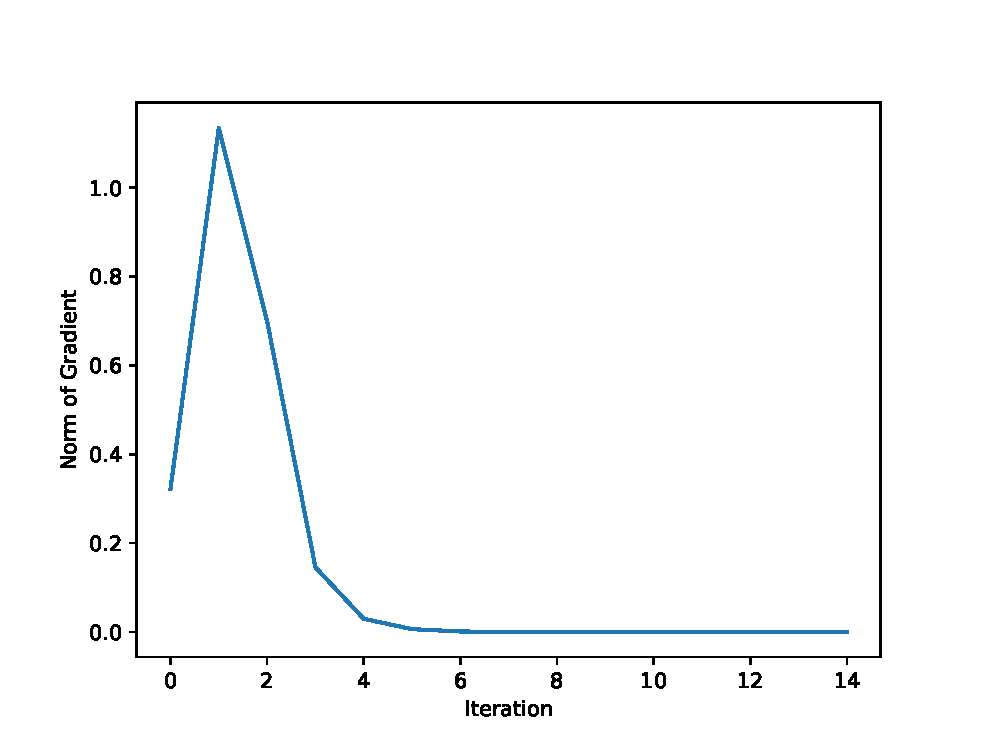
\includegraphics[width=\textwidth]{images/python/sd-pB.eps}
\caption{}
\label{fig:Class distribution}
\end{subfigure}
\hfill 
\begin{subfigure}[t]{0.4\textwidth}
\centering
    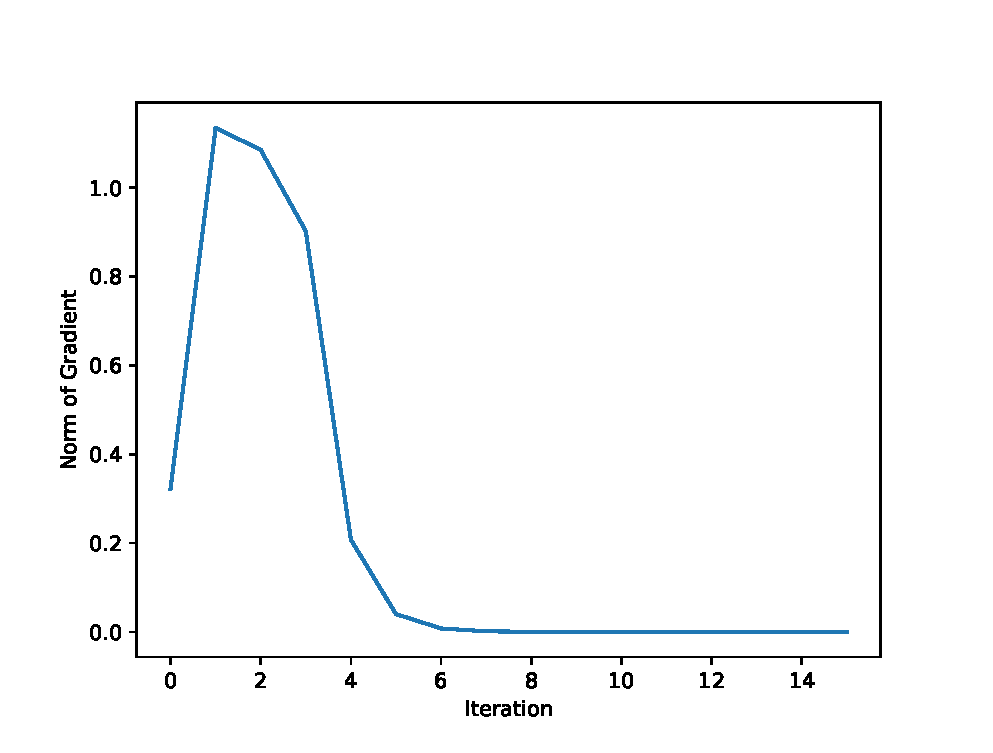
\includegraphics[width=\textwidth]{images/python/sec-pB.eps}
    \caption{}
    \label{fig:TSNE}
\end{subfigure}
\hfill
\begin{subfigure}[t]{0.4\textwidth}
\centering
    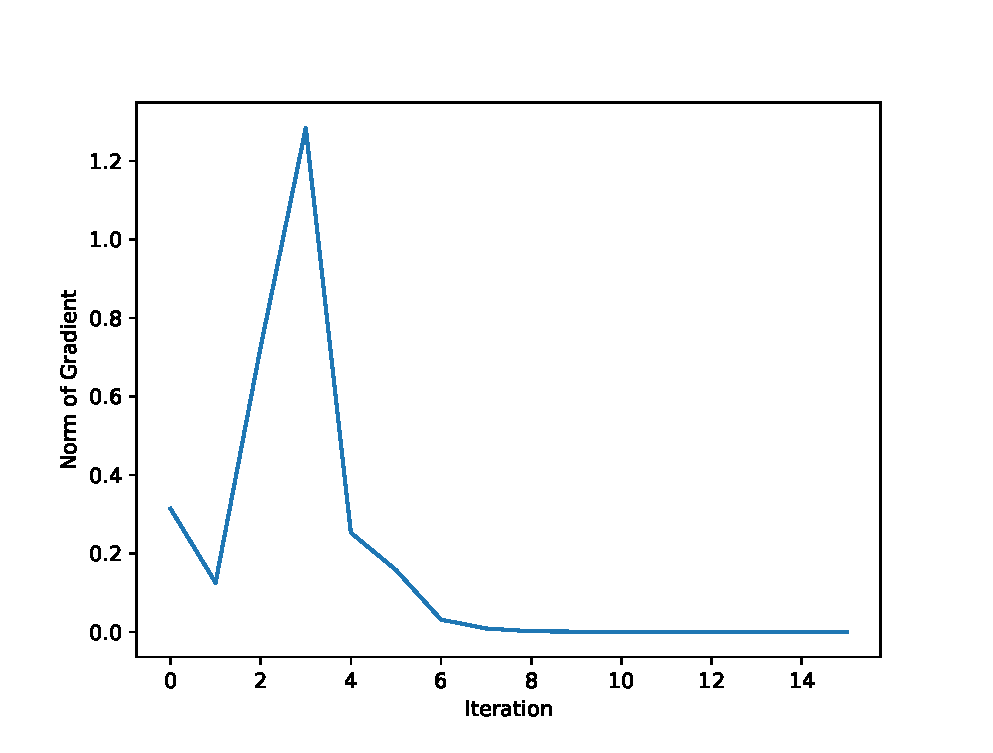
\includegraphics[width=\textwidth]{images/python/cg-pB.eps}
    \caption{}
    \label{fig:TSNE}
\end{subfigure}
\hfill
\begin{subfigure}[t]{0.4\textwidth}
\centering
    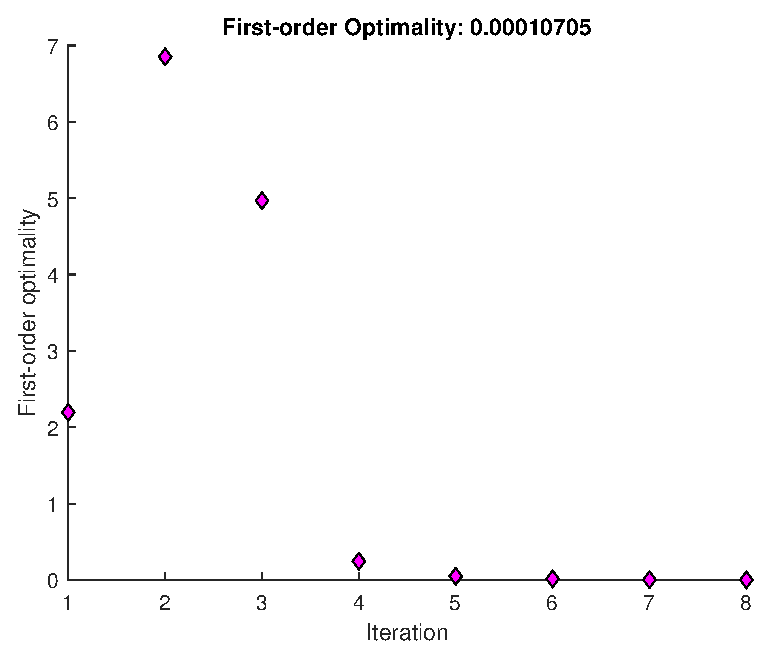
\includegraphics[width=\textwidth]{images/matlab/1c_loss.eps}  
    \caption{}
    \label{fig:TSNE}
\end{subfigure}
\caption{(a): Steepest descent, (b): Secant method, (c): Conjugate gradient, (d): Matlab: \textit{fminunc - quasi-newton method}}
\end{figure}
\begin{figure}
    \centering
    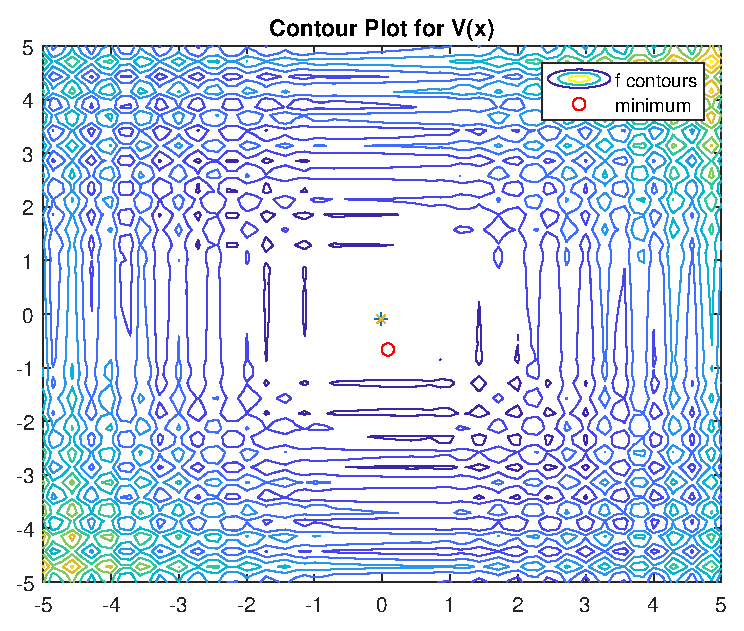
\includegraphics[width=0.4\textwidth]{images/matlab/matlab_1c.eps}
    \caption{Contour Plot for $V(x) = 1 + \left[ \begin{array}{cc} 1 & 2 \end{array} \right] x + \frac{1}{2} x^T \left[ \begin{array}{cc} 12 & 3 \\ 3 & 10 \end{array} \right] x  \hspace{2mm} + 10 \mbox{ln}(1+ x_1^4) \hspace{2mm}\mbox{sin}(100x_1)+ 10 \mbox{ln}(1+x_2^4) \mbox{cos}(100x_2)$}
\end{figure}

\clearpage
\section{Constrained Optimization}
\textbf{\subsection{Algorithms To Solve Constrained Nonlinear Programming Problem}}
\noindent There are different algorithms that can solve general nonlinear programming problems for equality constraints that include the following:
\begin{enumerate}
    \item Augmented Lagrangian Algorithm
    \item Lagrange - Newton Algorithm
    \item Penalty function algorithm
    \item Barrier function algorithm
\end{enumerate}
\subsubsection{Augmented Lagrangian methods}
The \textit{augmented Lagrangian function} is obtained by adding
a quadratic penalty term to the Lagrangian function, which gives the following.
\begin{equation}
    L_A(x, \lambda, \rho) \equiv f(x) - \lambda^Tc(x) + \frac{1}{2}\rho(x)^Tc(x)
\end{equation}
where $\rho$ is a non negative penalty parameter. Both the quadratic penalty term
of (12) and its gradient vanish at $x^*$. Thus, if $\lambda = \lambda^*$, $x^*$ is a stationary point (with respect to $x$) of (12). The Hessian matrix of the augmented Lagrangian function is
\begin{equation*}
    \nabla^2L_A(x,\lambda, \rho) = \nabla^2f(x) - \sum_{i=1}^{m} (\lambda_i - \rho c_i(x))\nabla^2c_i(x) + \rho A(x)^TA(x). 
\end{equation*}
Since $c(x^*)=0$, the Hessian of the penalty term at $x^*$ is simply $\rho A(x^*)^TA(x^*)$, which is a positive semi-definite matrix with strictly positive eigenvalues corresponding to the eigenvectors in the range of $A(x^*)^T$. Thus, the
presence of the penalty term in $L_A$ has the effect of increasing the (possibly negative) eigenvalues of $\nabla^2L(x^*, \lambda^*)$ corresponding to eigenvectors in the
range space of $A(x^*)^T$, but leaving the other eigenvalues unchanged. Using this
property, under mild conditions there exists a finite $\bar{\rho}$ such that $x^*$ is an
unconstrained minimizer of $L_A(x, \lambda^*, \rho)$ for all $\rho > \bar{rho}$.\\

In a typical augmented Lagrangian method, $x_k$ is taken as the unconstrained
minimizer of $L_A$ in (12), where $\lambda$ is taken as $\lambda_k$, the latest multiplier estimate. Strategies must therefore be developed for choosing both $\lambda_k$ and $\rho$.\\

\noindent Assume that the sufficient conditions for optimality hold at $x^*$. Then $x^*$ is a \textit{stationary point} of the Lagrangian function $L_A(x, \lambda = f(x) - \lambda^Tc(x)$, when $\lambda = \lambda^*$. Because $x^*$ is not necessarily a minimizer of the Lagrangian function, the Lagrangian function itself is not a suitable choice for the objective function of the subproblem, even if A* were known.\\

\noindent Since the \textit{reduced} Hessian of the Lagrangian function is positive definite,$x^*$ is a minimizer of the Lagrangian function within the subspace of vectors orthogonal to $A(x^*)$. The positive definiteness of the reduced Hessian of the Lagrangian function indicates that the Lagrangian function can display a negative curvature at $x^*$ only along directions in the range space of $A(x^*)^T$. This suggests that a suitable function for an unconstrained subproblem might be obtained by augmenting the Lagrangian function through the addition of a term that retains the stationary properties of $x^*$, but alters the Hessian in the range space of $A(x^*)^T$.\cite{KKT11, Haestene2, flect}

\subsubsection{Penalty Function Algorithm}
A penalty function method aims to replace a constrained optimization problem by using a series of unconstrained problems whose solutions converge to the solution of the constrained problem. The unconstrained problems are formed by adding a term, called a penalty function, to the objective function that consists of a penalty parameter multiplied by a measure of violation of the constraints.

\subsubsection{Barrier-function algorithms}
Barrier-function methods can be applied only to inequality constraints for which a strictly feasible initial point exists. Thereafter, a barrier function method generates a sequence of strictly feasible iterations. These methods have received enormous attention recently because of their close relationship with the "new" polynomial approaches to linear programming.\cite{Han111, Gill,Haestene2} \\
\indent In many physical and engineering applications, the constraint functions not only characterize the desired properties of the solution, but also define a region in which the problem statement is meaningful (for example, $f(x)$ or some of the constraint functions may be undefined outside the feasible region). An artificial convention to extend the problem statement outside the feasible region would not lend itself to the design of a computationally reasonable algorithm and might introduce complications not present in the original problem.\cite{Boyd111}\\
\indent Barrier-function methods require strict satisfaction of all constraints at the starting point and subsequent iterations. The continued enforcement of feasibility is the "opposite" of a penalty function method for inequalities, where the constrained solution is approached through a sequence of strictly \textit{infeasible} points with respect to the active constraints.  As in the penalty case, a barrier-function method creates a sequence of modified functions whose successive unconstrained minimizers should converge in the limit to the constrained solution. In general, the unconstrained minimizer of $f$ will be \textit{infeasible}, or $f$ may be unbounded below. In order to guarantee that successive iterates are feasible, the modified objective function includes a term to keep iterates "inside" the feasible region. If a "barrier" is created at the boundary of the feasible region by constructing a continuous function with a positive singularity, any unconstrained minimizer of the modified function must lie strictly inside the feasible region. If the weight assigned to the barrier term is decreased toward zero, the sequence of unconstrained minimizers should generate a strictly feasible approach to the constrained minimizer.\cite{Haestene2}
%






\subsection{Nonlinear Optimization problem}
The objective is to minimize the following cost function:
\begin{align}
(A) : \hspace{2mm}
& \mbox{minimize} \ V(x) = | x_1 -1 | + | x_2 - 2 | ; \ \  x =[x_1 \ x_2] \in \mathbb{R}^2 \nonumber \\
& \mbox{subject to : } \nonumber \\
& \hspace{2cm} h_1(x)= x_1 - x_2^2  \geq 0 \nonumber \\
& \hspace{2cm} h_2(x)= x_1^2 + x_2^2 -1  = 0 \nonumber
\end{align}
This is a constrained nonlinear optimization problem of the form:
\begin{align}
    minimize \hspace{2mm} V(x) = f(x) \\
    subject\hspace{2mm} to\hspace{2mm} c(x) \geq 0 \\
    subject\hspace{2mm} to \hspace{2mm}h(x) = 0 \\
\end{align}
This can be solved using these algorithms: 
\begin{itemize}
    \item Penalty Function Algorithm
    \item Barrier Function Algorithm
    \item Augmented Lagrangian Algorithm
    \item Lagrange-Newton Algorithm
\end{itemize}
\subsubsection{Solutions to constrained nonlinear problem using our python programs and matlab benchmark \textit{fmincon} function: }
The algorithms converged to very close local minimal solutions for $x$ with a tolerance set to be $tol =1e-8$ and the same initial value of all column vector of $[0,0]^{T}$ as confirmed in the contour plot in figure 7.
The gradient loss of the penalty function converged to its minima in 2 iterations while the augmented Lagrangian took longest to 15 iterations to converge; this might be due to the Hessian calculation. The Matlab implementation used sequential quadratic programming which approached the minimum at 2 iterations. 
The contour plot of the function $V(x)$ and the minimum solutions of $x$ derived from the algorithms showed that the lowest value of the objective function for the four algorithms lies at the intersection of the ellipse and the contour plot of the objective function. 
\begin{table}[htbp]
\centering
\begin{center}
\begin{tabular}{|c|c|c|c|c|}
\hline
 & \textbf{Penalty} &\textbf{Aug Lag} &\textbf{Newton Lag} & \textbf{Matlab}\\
\hline
Iterations & 3 &15& 5& 2\\
\hline
$x$ & 
\begin{bmatrix}
0.70703 \\
0.7073 \\
\end{bmatrix}
& \begin{bmatrix}
 0.7072 \\
 0.7073 \\
\end{bmatrix} &\begin{bmatrix}
   0.6180 \\
    0.7861 \\  
\end{bmatrix}
&\begin{bmatrix}
   0.7071 \\
    0.7071 \\  
\end{bmatrix} \\
\hline 
\end{tabular}
\label{table:results}
\caption{Algorithm performance}
\end{center}
\end{table}

\begin{figure}[h!]
\centering
\begin{subfigure}[t]{0.4\textwidth}
\centering
    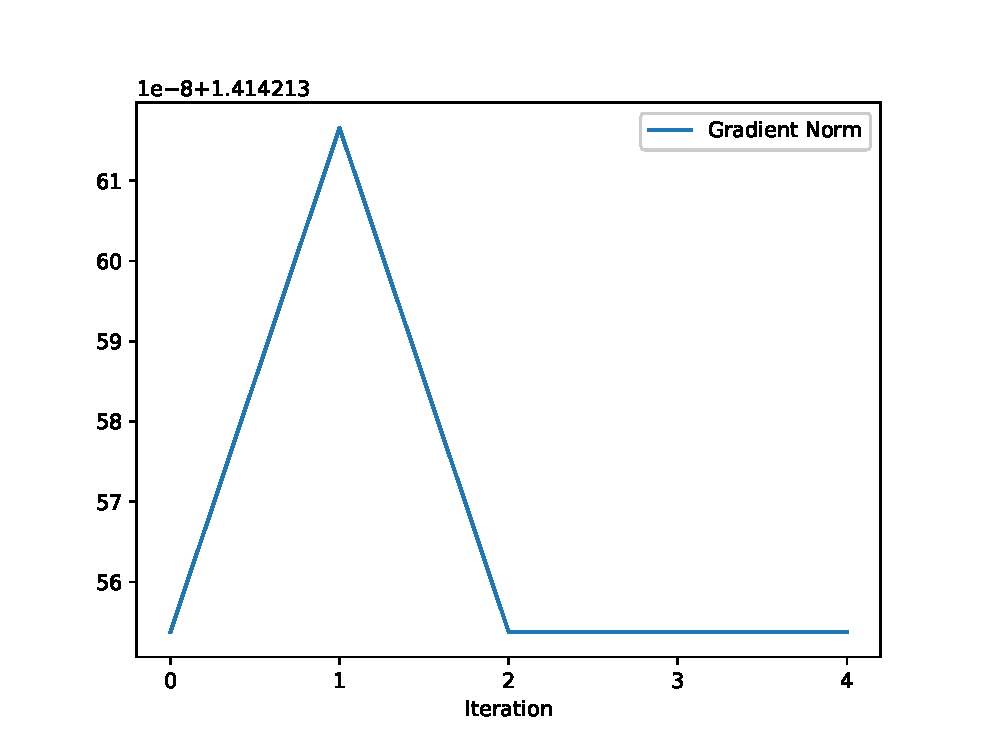
\includegraphics[width=\textwidth]{images/python/pe-pD.eps}
\caption{}
\end{subfigure}
\hfill 
\begin{subfigure}[t]{0.4\textwidth}
\centering
    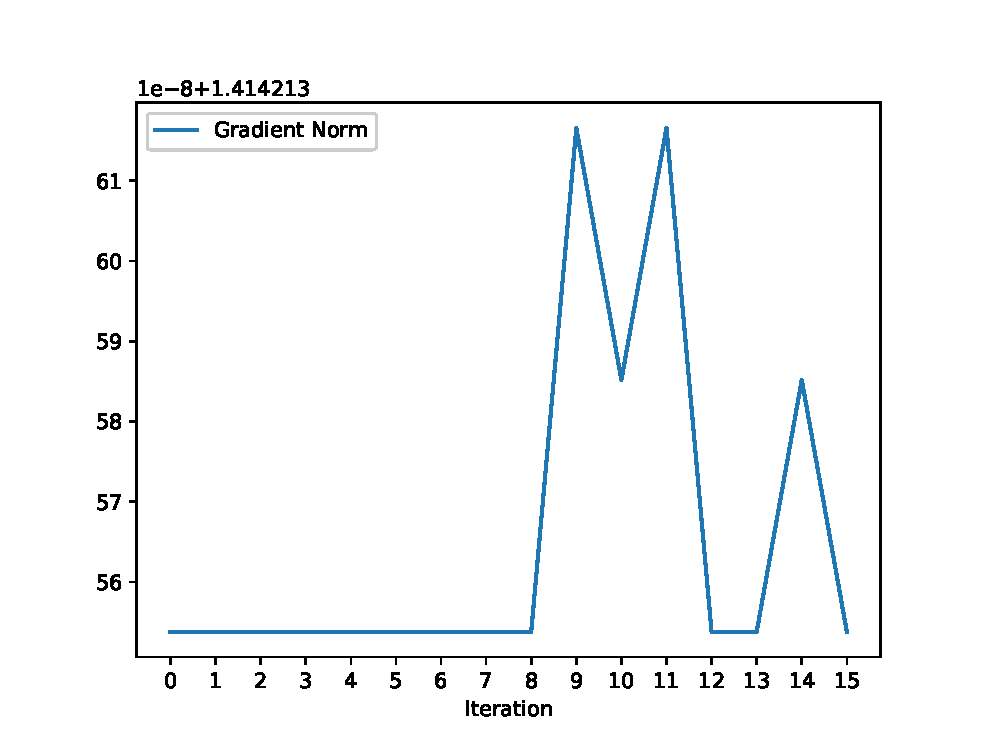
\includegraphics[width=\textwidth]{images/python/al-pD-ag.eps}
    \caption{}
\end{subfigure}
\hfill
\begin{subfigure}[t]{0.4\textwidth}
\centering
    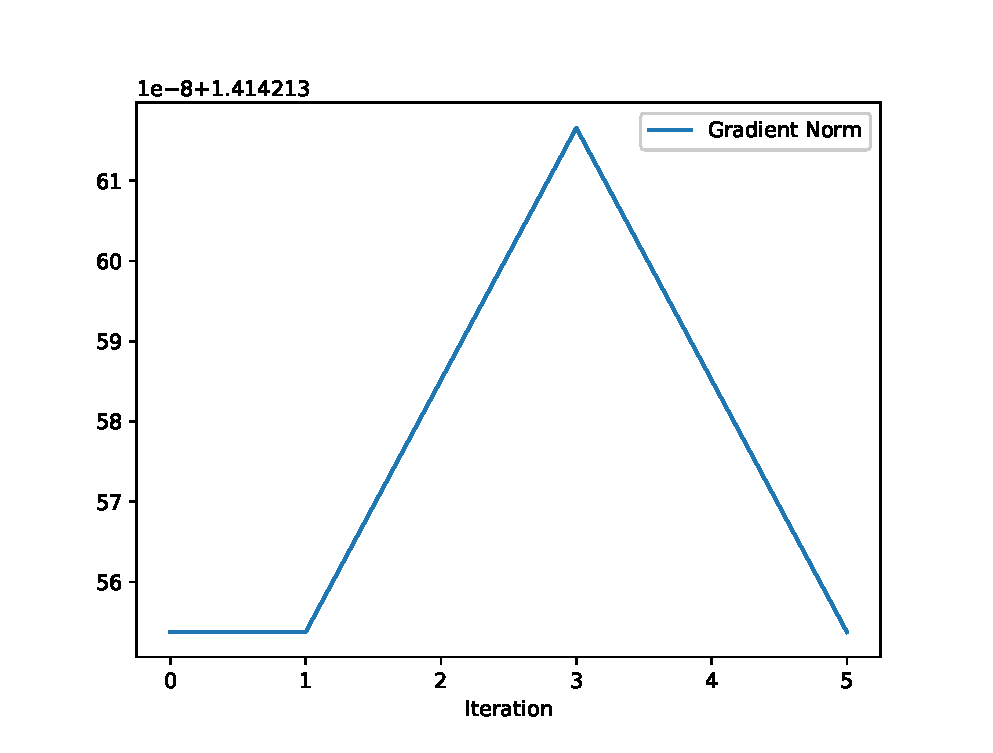
\includegraphics[width=\textwidth]{images/python/al-pD-ln.eps}
    \caption{}
\end{subfigure}
\hfill
\begin{subfigure}[t]{0.4\textwidth}
\centering
    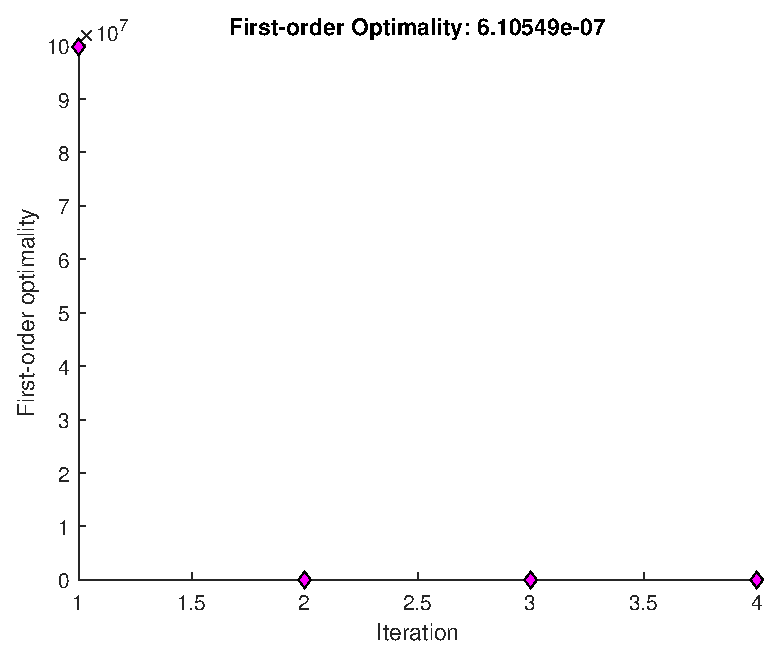
\includegraphics[width=\textwidth]{images/matlab/2a_loss.eps}
    \caption{}
\end{subfigure}
\caption{(a): Penalty, (b): Augmented Lagragrian, (c): Lagrangian, (d): Matlab: \textit{fmincon - sequential quadratic programming}}
\end{figure}
\begin{figure}
    \centering
    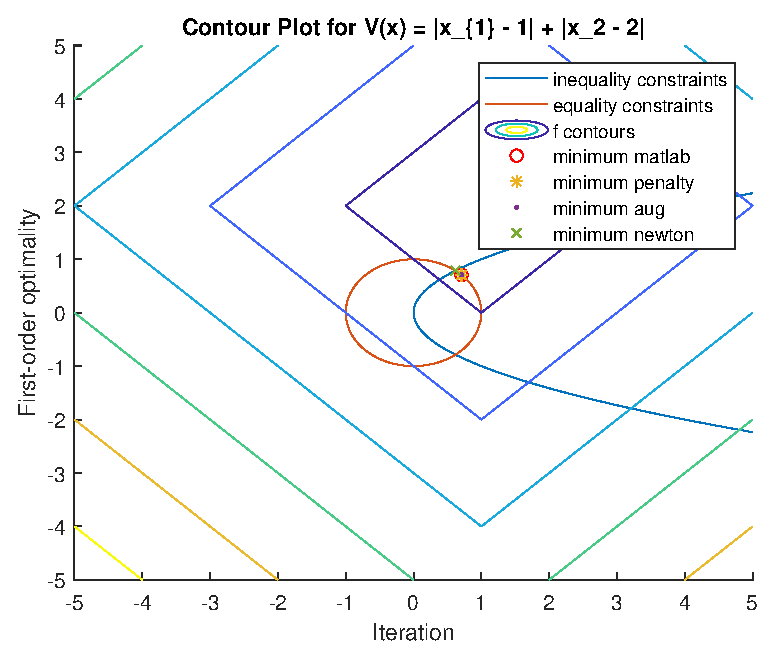
\includegraphics[width=0.4\textwidth]{images/matlab/matlab_2a.eps}
    \caption{Contour Plot for $V(x) =  | x_1 -1 | + | x_2 - 2 |$ and its constraints}
\end{figure}
\clearpage
\subsection{Nonlinear Optimization problem}
The objective is to minimize the following cost function:
\begin{align}
(B) : \hspace{2mm}
& \mbox{minimize} V (x) = - x_1 x_2 ; \ \  x \in \mathbb{R}^2 \nonumber \\
& \mbox{subject to : } \nonumber \\
& \hspace{2cm} h_1(x)= -x_1 - x_2^2 +1  \geq 0 \nonumber \\
& \hspace{2cm} h_2(x)= x_1 + x_2 \geq 0 \nonumber
\end{align}
This is a constrained nonlinear optimization problem of the form:
\begin{align}
    minimize \hspace{2mm} V(x) = f(x) \\
    subject\hspace{2mm} to\hspace{2mm} c(x) \geq 0 \\
    subject\hspace{2mm} to \hspace{2mm}h(x) = 0 \\
\end{align}
This can be solved using these algorithms: 
\begin{itemize}
    \item Penalty Function Algorithm
    \item Barrier Function Algorithm
    \item Augmented Lagragrian Algorithm
    \item Lagrange-Newton Algorithm
\end{itemize}
\subsubsection{Solutions to constrained nonlinear problem using our python programs and matlab benchmark \textit{fmincon} function: }
The algorithms converged to very close local minimal solutions for $x$ with a tolerance set to be $tol =1e-4$ and the same initial value of all column vector of $[5,5]^{T}$ as confirmed in the contour plot in figure 9.
The gradient loss of the penalty function converged to its minima in 2 iterations, while the newton Lagrangian took longest to converge using 3 iterations to converge. Unusually, our python solution converges faster than the matlab implementation that uses the interior point method. The solution from the newton Lagrangian and augmented newton method appears to be a long way off, as it lies on the intersections of the constraints of the contour plot. 
The contour graph of the function $V(x)$ and the minimum solutions of $x$ derived from the penalty algorithms showed that the lowest value of the objective function was at the intersection of the constraint ellipse and the contour graph of the objective function. 
\begin{table}[htbp]
\centering
\begin{center}
\begin{tabular}{|c|c|c|c|c|}
\hline
 & \textbf{Penalty} &\textbf{Aug Lag} &\textbf{Newton Lag} & \textbf{Matlab}\\
\hline
Iterations & 2 & 3 &2& 10 \\
\hline
$x$ & 
\begin{bmatrix}
0.6672 \\
0.5773 \\
\end{bmatrix}
&\begin{bmatrix}
 0.6178 \\
 -0.6182 \\
\end{bmatrix} &\begin{bmatrix}
 -1.6180 \\
 1.6180 \\
\end{bmatrix}
&\begin{bmatrix}
  0.6667 \\
 0.5774 \\
\end{bmatrix} \\ 
\hline 
\end{tabular}
\label{table:results}
\caption{Algorithm performance}
\end{center}
\end{table}

\begin{figure}[h!]
\centering
\begin{subfigure}[t]{0.4\textwidth}
\centering
    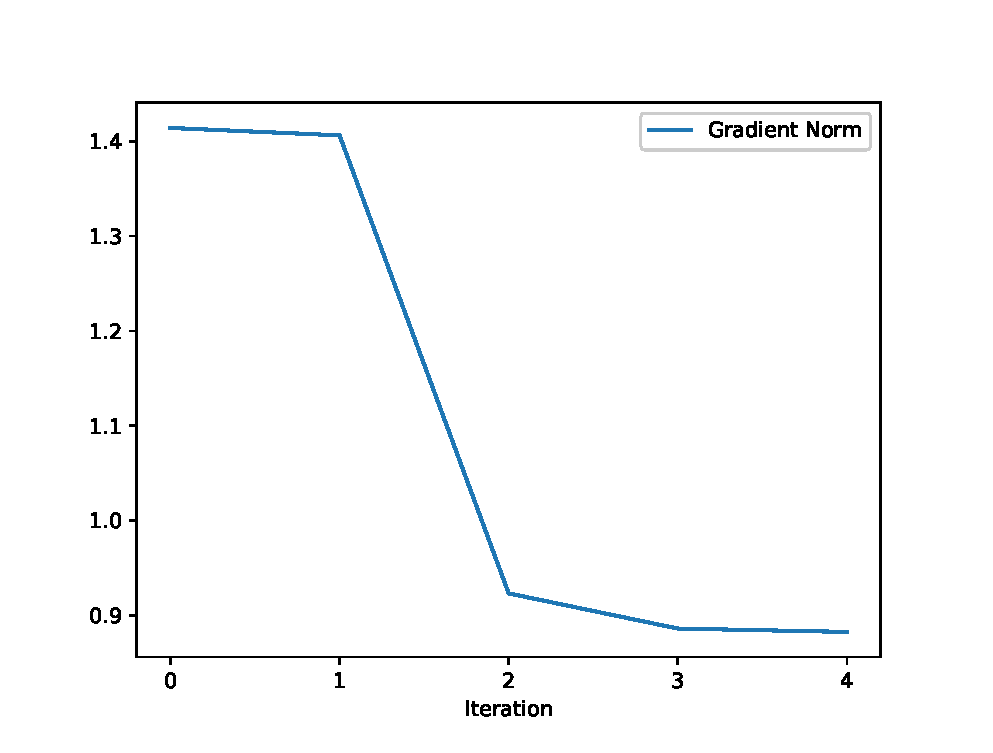
\includegraphics[width=\textwidth]{images/python/pe-pE.eps}
\caption{}
\label{fig:Class distribution}
\end{subfigure}
\hfill 
\begin{subfigure}[t]{0.4\textwidth}
\centering
    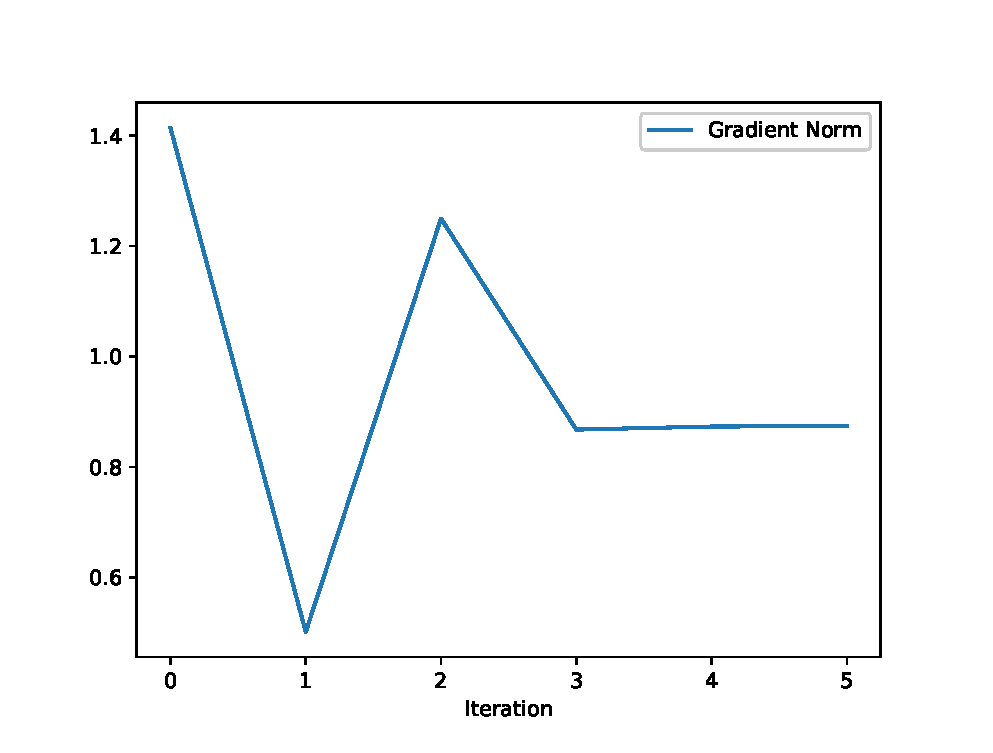
\includegraphics[width=\textwidth]{images/python/al-pE-ag.eps}
    \caption{}
    \label{fig:TSNE}
\end{subfigure}
\hfill
\begin{subfigure}[t]{0.4\textwidth}
\centering
    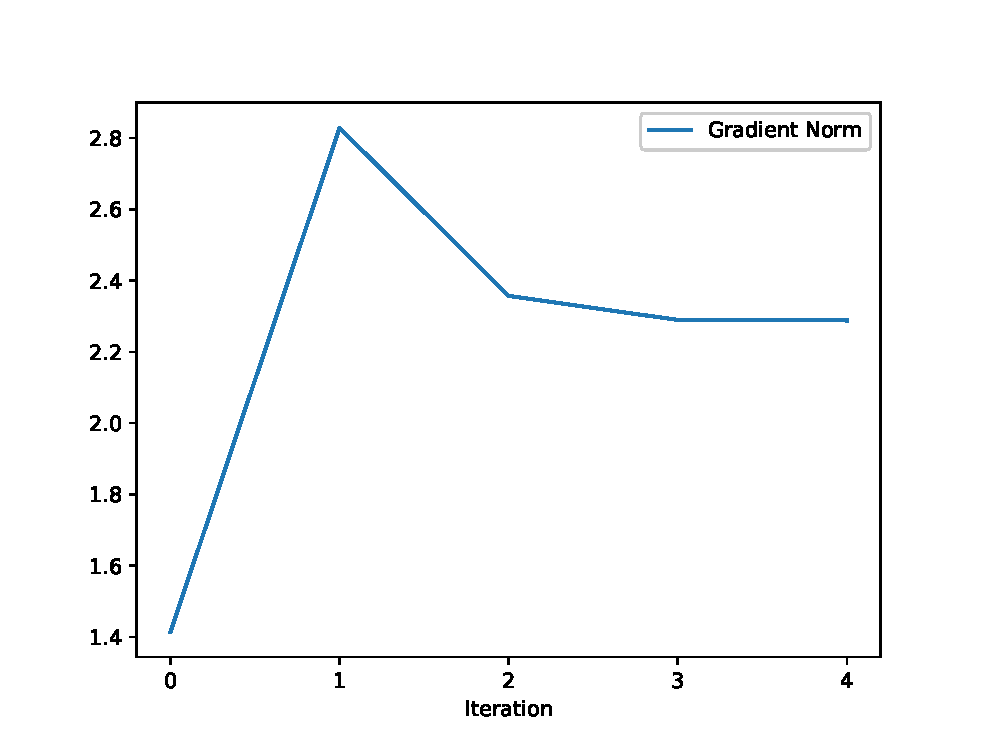
\includegraphics[width=\textwidth]{images/python/al-pE-ln.eps}
    \caption{}
    \label{fig:TSNE}
\end{subfigure}
\hfill
\begin{subfigure}[t]{0.4\textwidth}
\centering
    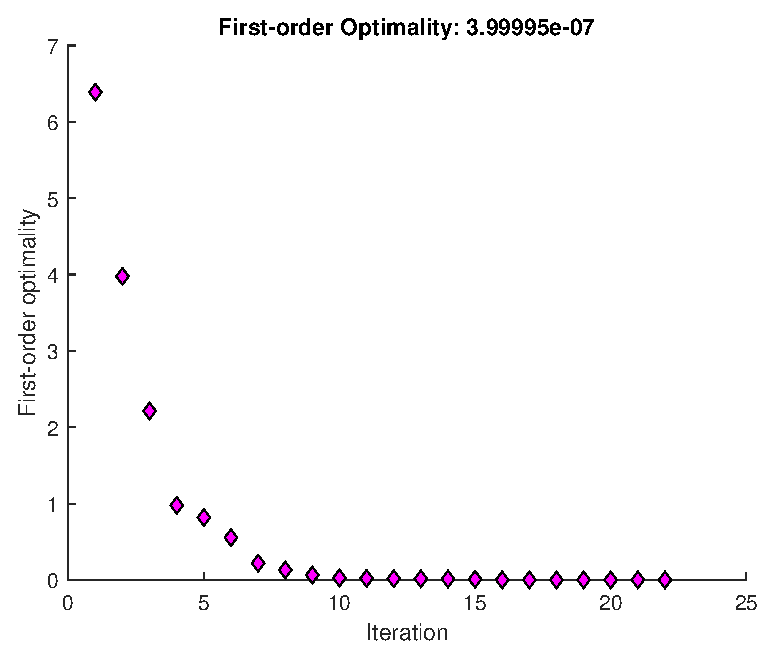
\includegraphics[width=\textwidth]{images/matlab/2b_loss.eps}
    \caption{}
    \label{fig:TSNE}
\end{subfigure}
\caption{(a): Penalty, (b): Augmented Lagrangian, (c): Newton Lagrangian, (d): Matlab: \textit{fmincon - interior - point}}
\end{figure}
\begin{figure}
    \centering
    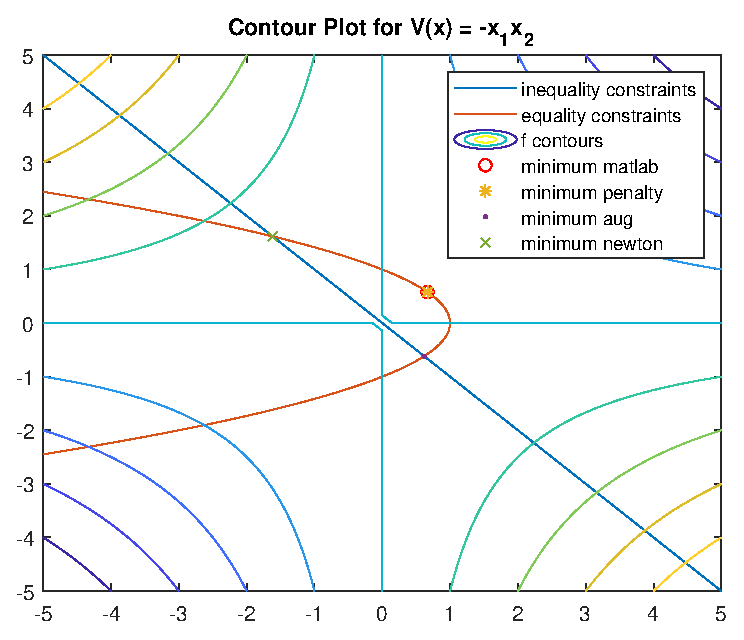
\includegraphics[width=0.4\textwidth]{images/matlab/matlab_2b.eps}
    \caption{Contour Plot for $V(x) =  V(x) = - x_1 x_2$ and its constraints}
\end{figure}
\clearpage
\subsection{Nonlinear Optimization problem}
The objective is to minimize the following cost function:
\begin{align}
(C) : \hspace{2mm}
& \mbox{minimize} \ V(x) = \mbox{ln}(x_1)- x_2 ; \ \  x \in \mathbb{R}^2 \nonumber \\
& \mbox{subject to : } \nonumber \\
& \hspace{2cm} h_1(x)= x_1 - 1  \geq 0 \nonumber \\
& \hspace{2cm} h_2(x)= x_1^2 + x_2^2 -4 = 0 \nonumber
\end{align}
This is a constrained nonlinear optimization problem of the form:
\begin{align}
    minimize \hspace{2mm} V(x) = f(x) \\
    subject\hspace{2mm} to\hspace{2mm} c(x) \geq 0 \\
    subject\hspace{2mm} to \hspace{2mm}h(x) = 0 \\
\end{align}
This can be solved using these algorithms: 
\begin{itemize}
    \item Penalty Function Algorithm
    \item Barrier Function Algorithm
    \item Augmented Lagragrian Algorithm
    \item Lagrange-Newton Algorithm
\end{itemize}
\subsubsection{Solutions to constrained nonlinear problem using our python programs and matlab benchmark \textit{fmincon} function: }
We encountered infeasible solutions full of zeros for this problem with the penalty function and augmented Lagrangian methos. The solution from the Lagrange-Newton Algorithm is very close local minimal solutions for $x$ with a tolerance set to be $tol =1e-8$ and the same initial value of all column vector of $[5,5]^{T}$ as confirmed in the contour plot in figure 11. Surprisingly, the gradient loss of the newton Lagrangian algorithm increases but settles after 2 iterations. The Matlab implementation used the quasi-Newton method approaching the minimum at 8 iterations.
The contour plot of the function $V(x)$ and the minimum solutions of $x$ derived from the newton Lagrangian algorithms showed that the lowest value of the objective function for at the intersection of the constraint ellipse and the contour plot of the objective function. 
\begin{table}[htbp]
\centering
\begin{center}
\begin{tabular}{|c|c|c|}
\hline
 &\textbf{\textit{Newton Lag}} & \textbf{Matlab}\\
\hline
Iterations & 27 & 82 \\
\hline
$x$ & 
\begin{bmatrix}
1 \\
1.732 \\
\end{bmatrix}
&\begin{bmatrix}
 1.0000  \\  1.7321 \\
\end{bmatrix}\\
\hline 
\end{tabular}
\label{table:results}
\caption{Algorithm performance}
\end{center}
\end{table}

\begin{figure}[h!]
\hfill
\begin{subfigure}[t]{0.4\textwidth}
\centering
    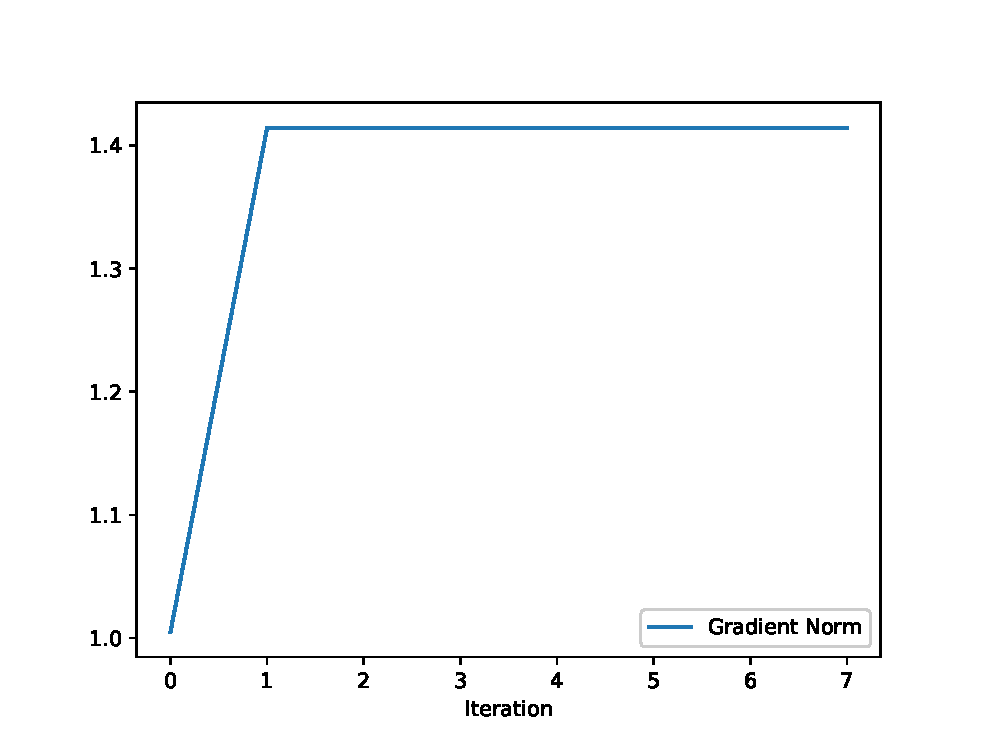
\includegraphics[width=\textwidth]{images/python/al-pF-ln.eps}
    \caption{}
    \label{fig:TSNE}
\end{subfigure}
\hfill
\begin{subfigure}[t]{0.4\textwidth}
\centering
    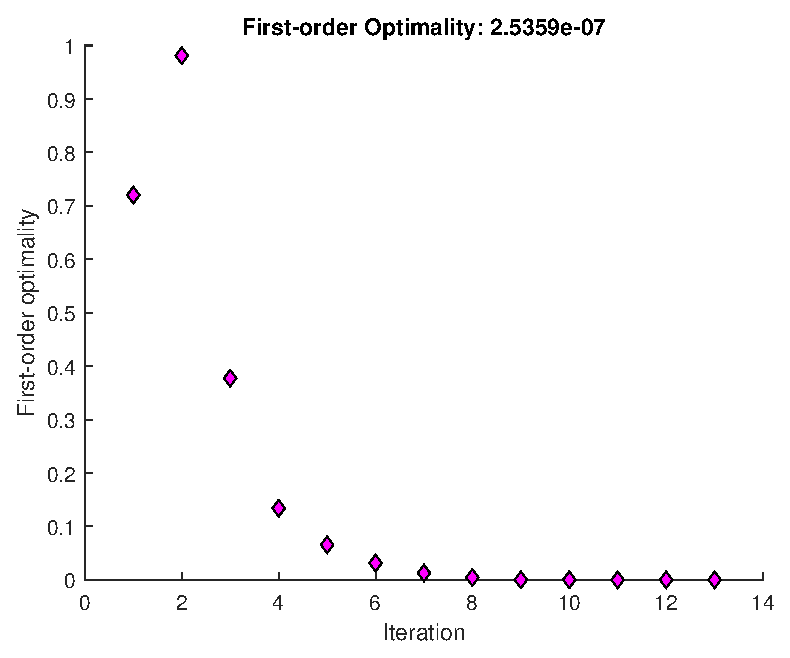
\includegraphics[width=\textwidth]{images/matlab/2c_loss.eps}
    \caption{}
    \label{fig:TSNE}
\end{subfigure}
\caption{(a): Newton Lagrangian, (d): Matlab: \textit{fmincon - interior - point}}
\end{figure}
\begin{figure}
    \centering
    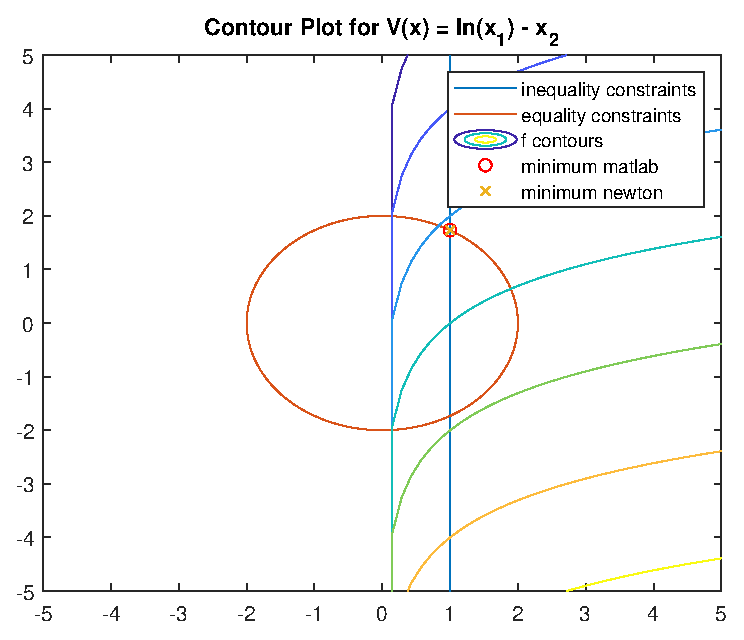
\includegraphics[width=0.4\textwidth]{images/matlab/matlab_2c.eps}
    \caption{Contour Plot for $V(x) =  V(x) = \mbox{ln}(x_1)- x_2$ and its constraints}
\end{figure}

\clearpage
\section{Discussion}
We successfully implemented all the algorithms in Python for the nonlinear optimization problems required and used them to solve constrained and unconstrained optimization problems, with very encouraging results, which could be made better with better algorithm implementation and test cases. \\
For the constrained nonlinear problems, we were not able to efficiently implement the barrier function algorithm as we continued to approach infeasible solutions full of zeros from various initial points.
\newpage
\addcontentsline{toc}{section}{References}
\bibliographystyle{ieeetr}
\bibliography{ref}
\nocite{*}
\clearpage
\section{Appendix : Code Listings}
\begin{lstlisting}
---------------------------Optimization Utils ----------------
import numpy as np

def get_step_size(p, x, s, gamma=1.5, mu=0.8):
    """
    Determines the step size using Armijo algorithm
    :param p: Problem
        The problem to be optimized
    :param x: numpy 2D array
        The point we are at
    :param s: numpy 2D array
        Search direction
    :param gamma: float
        Parameter for increasing step size
    :param mu: float
        Parameter for decreasing step size
    :return: float
        Step size
    """
    w = 1  # Default step size

    k_g = 0  # Power of gamma
    k_m = 0  # Power of mu

    # Precompute cost and gradient to save time
    vx = p.get_cost(x)
    gx_s = p.get_grad(x) @ s

    def v_bar(w):
        return vx + 0.5 * w * gx_s

    while p.get_cost(x + gamma ** k_g * s) < v_bar(gamma ** k_g):
        k_g += 1
        w = gamma ** k_g

    while p.get_cost(x + mu ** k_m * gamma ** k_g * s) > v_bar(mu ** k_m * gamma ** k_g):
        k_m += 1
        w = mu ** k_m * gamma ** k_g

    return w

def check_cone_condition(p, x, s, theta=89):
    """
    Checks the cone condition at a point
    :param p: Problem
        The problem to be optimized
    :param x: numpy 2D array
        The point we are at
    :param s: numpy 2D array
        Search direction
    :param theta: float
        Acceptable angle with gradient in degrees
    :return: bool
        True if s within theta degrees of gradient at x
    """
    gx = p.get_grad(x)  # get gradient at x
    cos_phi = (-gx @ s) / (np.linalg.norm(s) * np.linalg.norm(gx))
    cos_theta = np.cos(theta * 2 * np.pi / 360)

    return (cos_phi > cos_theta)

def get_cost_norm(p, x):
    """
    Evaluates the cost at d
    :param p: Problem
        The problem to be optimized
    :param x: numpy 2D array
        The point at which we want to get the cost
    :return: float
        The cost at x
    """
    cost = 0
    if p.get_eq_const() is not None:
        cost = cost + np.linalg.norm(p.get_eq_const(x))**2
    if p.get_ineq_const() is not None:
        ineq_x = p.get_ineq_const(x)
        c = np.minimum(np.zeros(np.shape(ineq_x)), ineq_x)
        cost = cost + np.linalg.norm(c)**2
    return np.sqrt(cost)

def get_fd_hessian(f, x, h=1e-8):
    """
    The finite difference approximation of the Hessian at x
    :param f: function of x
        Function whose Hessian we want to evaluate
    :param x: numpy 2D array
        Point at whihc we want to evaluate the Hessian
    :param h: float
        Step size
    :return: 2D numpy matrix
        Hessian at x
    """
    dim = np.max(np.shape(x))
    I = np.eye(dim)
    H = np.zeros((dim, dim))

    for i in range(0, dim):
        for j in range(0, dim):
            H[i, j] = (f(x + h * I[:, [i]] + h * I[:, [j]]) \
                       - f(x + h * I[:, [i]]) - f(x + h * I[:, [j]]) \
                       + f(x)) / h ** 2

    return 0.5 * (H + H.T)

def get_fd_grad(f, x, h=1e-8):
    """
    Finite difference approximation of gradient at x
    :param f: function of x
        function whose gradient we want to evaluate
    :param x: numpy 2D array
        point at which we want to approximate the gradient
    :param h: float
        step size
    :return: numpy 2D array
        gradient at x 
    """
    dim = np.max(np.shape(x))
    grad_gen = ((f(x + h * np.eye(dim)[:, [i]]) - f(x)) / h
                for i in range(0, dim))
    grad = np.expand_dims(np.fromiter(grad_gen, np.float64), axis=0)
    return grad

--------------------------------------Optimization------------------------------------------
import numpy as np
from functools import partial
from optimization_utils import get_step_size,check_cone_condition,get_cost_norm,get_fd_hessian,get_fd_grad

class Problem:
    """
    This class defines an optimization problem
    """
    def __init__(self, cost, grad='fd', grad_step=1e-8,
                 eq_const=None, ineq_const=None):
        """
        Constructor for the otpimization problem

        :param cost: function with 2D NumPy array as input
            Objective function of the problem
        :param grad: function with 2D NumPy array as input
            Gradient function of the problem.
            Default = 'fd', finite difference used
        :param grad_step: float
            Step size for finite difference gradient.
            Only required if :param grad= 'fd'.
            Default = 1e-8
        :param eq_const: list of functions
            Equality constraints of the problem
        :param ineq_const: list of functions
            Inequality constraints of the problem
        """
        self._cost = cost

        if grad == 'fd':
            # finite difference method specified
            self._grad_step = grad_step  # default 1e-8
            self._grad = partial(get_fd_grad, self.get_cost, h=self._grad_step)

        else:
            # gradient specified, don't need step size
            self._grad_step = None
            self._grad = grad

        self._eq_const = eq_const
        self._ineq_const = ineq_const

    def get_cost(self, x=None):
        """
        Returns the cost of the problem if x is specified.
        Else, returns the cost function.

        :param x: 2D numpy array
            Point at which the cost is calculated.
            Default = None
        :return: function or float
            If x is None, returns the cost function.
            Else, returns the cost at x.
        """
        if x is not None:
            return self._cost(x)
        else:
            return self._cost

    def get_grad(self, x=None):
        """
        Returns the gradient of the problem if x is specified.
        Else, returns the gradient function.

        :param x: 2D numpy array
            Point at which the gradient is calculated.
            Default = None
        :return: function or float
            If x is None, returns the gradient function.
            Else, returns the gradient at x.
        """
        if x is not None:
            return self._grad(x)
        else:
            return self._grad

    def get_eq_const(self, x=None):
        """
        Equality constraints of the problem.
        If x is None, returns an array of functions.
        Else, returns an array of equality constraints evaluated at x

        :param x: 2D numpy array
            Point at which the equality constraints are evaluated.
        :return: 2D numpy array
            Array of functions if x = None.
            Else, array of equality constraints evaluated at x
        """
        if self._eq_const is not None:
            if x is not None:
                return np.array([[eq(x)] for eq in self._eq_const])
            else:
                return np.array([eq for eq in self._eq_const])
        else:
            return None

    def get_ineq_const(self, x=None):
        """
        Inequality constraints of the problem.
        If x is None, returns an array of functions.
        Else, returns an array of inequality constraints evaluated at x

        :param x: 2D numpy array
            Point at which the inequality constraints are evaluated.
        :return: 2D numpy array
            Array of functions if x = None.
            Else, array of inequality constraints evaluated at x
        """
        if self._ineq_const is not None:
            if x is not None:
                return np.array([[ineq(x)] for ineq in self._ineq_const])
            else:
                return np.array([ineq for ineq in self._ineq_const])
        else:
            return None

    def num_eq_const(self):
        """
        The number of equality constraints.

        :return: int
            The number of equality constraints.
        """
        if self._eq_const is not None:
            return np.max(np.shape(self._eq_const))
        else:
            return 0

    def num_ineq_const(self):
        """
        The number of inequality constraints.

        :return: int
            The number of inequality constraints.
        """
        if self._ineq_const is not None:
            return np.max(np.shape(self._ineq_const))
        else:
            return 0

def steepest_descent(p, x, tol=1e-6, max_iter=999, hist=False):
    """
    Steepest Descent algorithm

    :param p: Problem
        Optimization problem to minimize
    :param x: 2D numpy array
        Initial guess
    :param tol: float
        Tolerance of the algorithm. If norm of gradient is less than tol,
        iterations stop.
        Default = 1e-6
    :param max_iter: int
        Maximum number of iterations before stopping
        Default = 999
    :param hist: bool
        Flag to return history of x or not
        Default = False
    :return: 2D or 3D numpy array
        If hist = False, returns the last value of x.
        Else, returns an array with values of x after each iteration
    """
    i = 0
    x_hist = []
    while np.linalg.norm(p.get_grad(x)) > tol:
        if i > max_iter:
            break
        s = -p.get_grad(x).T # get the gradient at x
        w = get_step_size(p, x, s) # get step size using Armijo algorithm
        x_hist.append(x)
        x = x + w * s # gradient descent
        i += 1 # increment iteration

    return x if not hist else np.array(x_hist)

def conjugate_gradient(p, x, tol=1e-6, rst_iter=99, max_iter=999, hist=False):
    """
    Conjugate gradient algorithm

    :param p: Problem
        Optimization problem to minimize
    :param x: 2D numpy array
        Initial guess
    :param tol: float
        Tolerance of the algorithm. If norm of gradient is less than tol,
        iterations stop.
        Default = 1e-6
    :param rst_iter: int
        Number of iterations before resetting search direction
        and restarting
        Default = 99
    :param max_iter: int
        Maximum total number of iterations
        Default = 999
    :param hist: bool
        Flag to return history of x or not
        Default = False
    :return: 2D or 3D numpy array
        If hist = False, returns the last value of x.
        Else, returns an array with values of x after each iteration
    """
    i = 0
    x_hist = []
    s = -p.get_grad(x).T
    while np.linalg.norm(p.get_grad(x)) > tol:
        if i > rst_iter or not check_cone_condition(p, x, s):
            i = 0
            s = -p.get_grad(x).T # get gradient at x
        # elif not check_cone_condition(p, x, s):
        #     i = 0
        #     s = -p.grad(x).T # get gradient at x
        elif i > max_iter:
            break
        w = get_step_size(p, x, s) # get step size using Armijo algorithm
        x_prv = x
        x_hist.append(x)
        x = x_prv + w * s
        beta = ((p.get_grad(x) - p.get_grad(x_prv)) @ p.get_grad(x).T) \
            / (p.get_grad(x_prv) @ p.get_grad(x_prv).T)
        s = -p.get_grad(x).T + beta * s
        i += 1

    return x if not hist else np.array(x_hist)

def secant(p, x, tol=1e-6, H=None, rst_iter=99, max_iter=999, hist=False):
    """
    Secant optimization algorithm

    :param p: Problem
        Optimization problem to minimize
    :param x: 2D numpy array
        Initial guess
    :param tol: float
        Tolerance of the algorithm. If norm of gradient is less than tol,
        iterations stop.
        Default = 1e-6
    :param H: 2D numpy matrix
        Initial guess at Hessian. If None, set to identity
        Default = None
    :param rst_iter: int
        Number of iterations before resetting search direction
        and restarting
        Default = 99
    :param max_iter: int
        Maximum total number of iterations
        Default = 999
    :param hist: bool
        Flag to return history of x or not
        Default = False
    :return: 2D or 3D numpy array
        If hist = False, returns the last value of x.
        Else, returns an array with values of x after each iteration
    """
    if H is None:
        H = np.eye(np.max(np.shape(x)))

    i = 0
    x_hist = []
    while np.linalg.norm(p.get_grad(x)) > tol:
        s = -H @ p.get_grad(x).T
        if i > rst_iter or not check_cone_condition(p, x, s):
            i = 0
            s = -p.get_grad(x).T # get gradient at x
        # elif not check_cone_condition(p, x, s):
        #     i = 0
        #     s = -p.grad(x).T
        elif i > max_iter:
            break
        w = get_step_size(p, x, s)
        x_prv = x
        x_hist.append(x)
        x = x_prv + w * s
        # Davidon-Fletcher-Powell (DFP) Algorithm
        dx = x - x_prv
        dg = p.get_grad(x) - p.get_grad(x_prv)
        H = H + (dx @ dx.T) / (dx.T @ dg.T) \
            - ((H @ dg.T) @ (H @ dg.T).T) / (dg @ H @ dg.T)
        i += 1

    return x if not hist else np.array(x_hist)

def penalty_function(p, x0, tol=1e-6, tol_cost=1e-4, sigma_max=1e6, hist=False):
    """
    Constrained optimization algorithm using penalty functions
    :param p: Problem
        Constrained optimization problem to minimize
    :param x0: 2D numpy array
        Initial guess
    :param tol: float
        Tolerance of the algorithm. If norm of gradient is less than tol,
        iterations stop.
        Default = 1e-6
    :param tol_cost: float
        Tolerance of cost. If norm of cost is less than tol_cost,
        iteration stops.
        Default = 1e-4
    :param sigma_max: float
        Maximum value of sigma before iteration stops
        Default = 1e6
    :param hist: bool
        Flag to return history of x or not
        Default = False
    :return: 2D or 3D numpy array
        If hist = False, returns the last value of x.
        Else, returns an array with values of x after each iteration
    """

    def phi(p, sigma, x):
        cost = p.get_cost(x) # get cost at x
        if p.get_eq_const() is not None:
            cost = cost + 0.5 * sigma * np.linalg.norm(p.get_eq_const(x))**2
        if p.get_ineq_const() is not None:
            ineq_x = p.get_ineq_const(x)
            c = np.minimum(np.zeros(np.shape(ineq_x)), ineq_x)
            cost = cost + 0.5 * sigma * np.linalg.norm(c)**2
        return cost

    # def cost_norm(x):
    #     cost = 0
    #     if p.eq_const() is not None:
    #         cost = cost + np.linalg.norm(p.eq_const(x))**2
    #     if p.ineq_const() is not None:
    #         ineq_x = p.ineq_const(x)
    #         c = np.minimum(np.zeros(np.shape(ineq_x)), ineq_x)
    #         cost = cost + np.linalg.norm(c)**2
    #     return np.sqrt(cost)

    sigma = 1
    x = x0 # initialize first guess
    x_hist = []

    while get_cost_norm(p, x) > tol_cost:
        up = Problem(partial(phi, p, sigma))
        x_hist.append(x)
        x = steepest_descent(up, x0, tol=tol)
        if sigma >= sigma_max:
            break
        sigma *= 10

    return x if not hist else np.array(x_hist)

def barrier_function(p, x0, tol=1e-6, tol_const=1e-4, sigma_max=1e6,
                     r_min=1e-6, mode='inv', hist=False):
    """
    Constrained optimization algorithm using barrier functions
    :param p: Problem
        Constrained optimization problem to minimize
    :param x0: 2D numpy array
        Initial guess
    :param tol: float
        Tolerance of the algorithm. If norm of gradient is less than tol,
        iterations stop.
        Default = 1e-6
    :param tol_cost: float
        Tolerance of cost. If norm of cost is less than tol_cost,
        iteration stops.
        Default = 1e-4
    :param sigma_max: float
        Maximum value of sigma before iteration stops
        Default = 1e6
    :param r_min: float
        Minimum value of r before iteration stops
        Default = 1e-6
    :param mode: String
        Mode of barrier function. 'inv' for inverse barrier function
        or 'log' for logarithmic barrier function
    :param hist: bool
        Flag to return history of x or not
        Default = False
    :return: 2D or 3D numpy array
        If hist = False, returns the last value of x.
        Else, returns an array with values of x after each iteration
    """
    def phi(p, sigma, r, x):
        cost = p.get_cost(x)
        if p.get_eq_const() is not None:
            cost = cost + 0.5 * sigma * np.linalg.norm(p.get_eq_const(x))**2
        if p.get_ineq_const() is not None:
            ineq_x = p.get_ineq_const(x)
            if mode == 'log':
                cost = cost - r * np.sum(np.log(ineq_x))
            else:
                cost = cost + r * np.sum(np.reciprocal(ineq_x))
        return cost

    # def cost_norm(x):
    #     cost = 0
    #     if p.eq_const() is not None:
    #         cost = cost + np.linalg.norm(p.eq_const(x))**2
    #     if p.ineq_const() is not None:
    #         ineq_x = p.ineq_const(x)
    #         c = np.minimum(np.zeros(np.shape(ineq_x)), ineq_x)
    #         cost = cost + np.linalg.norm(c)**2
    #     return np.sqrt(cost)

    sigma = 1
    r = 1
    x = x0
    x_hist = []

    while get_cost_norm(p, x) > tol_const:
        up = Problem(partial(phi, p, sigma, r))
        x_hist.append(x)
        x = steepest_descent(up, x0, tol=tol)
        if sigma >= sigma_max or r <= r_min:
            break
        sigma *= 10
        r *= 0.1

    return x if not hist else np.array(x_hist)

def augmented_lagrange(p, x0, tol=1e-6, tol_cost=1e-6, sigma_max=1e12, hist=False):
    """
    Constrained optimization algorithm using augmented Lagrange method
    :param p: Problem
        Constrained optimization problem to minimize
    :param x0: 2D numpy array
        Initial guess
    :param tol: float
        Tolerance of the algorithm. If norm of gradient is less than tol,
        iterations stop.
        Default = 1e-6
    :param tol_cost: float
        Tolerance of cost. If norm of cost is less than tol_cost,
        iteration stops.
        Default = 1e-6
    :param sigma_max: float
        Maximum value of sigma before iteration stops
        Default = 1e6
    :param hist: bool
        Flag to return history of x or not
        Default = False
    :return: 2D or 3D numpy array
        If hist = False, returns the last value of x.
        Else, returns an array with values of x after each iteration
    """
    def phi(p, lmb, sgm, x):
        cost = p.get_cost(x)

        n_e = p.num_eq_const()
        n_i = p.num_ineq_const()
        n_c = n_e + n_i

        lmb_e = lmb[0:n_e, :]
        lmb_i = lmb[n_e:n_c, :]
        sgm_e = sgm[0:n_e, :]
        sgm_i = sgm[n_e:n_c, :]

        if p.get_eq_const() is not None:
            c_e = p.get_eq_const(x)
            cost = cost - sum(lmb_e * c_e) + 0.5 * sum(sgm_e * c_e**2)

        if p.get_ineq_const() is not None:
            c_i = p.get_ineq_const(x)
            p_i = np.array([-lmb_i[i] * c_i[i] + 0.5 * sgm_i[i] * c_i[i]**2 \
                            if c_i[i] <= lmb_i[i] / sgm_i[i] \
                            else -0.5 * lmb_i[i]**2 / sgm_i[i] \
                            for i in range(0, n_i)])
            cost = cost + sum(p_i)

        return cost

    x_hist = []

    n_e = p.num_eq_const()
    n_i = p.num_ineq_const()
    n_c = n_e + n_i

    lmb = np.zeros((n_c, 1))
    sgm = np.ones((n_c, 1))

    x = x0
    c = 1e12 * np.ones((n_c, 1))

    while np.linalg.norm(c) > tol_cost:
        # Create new problem to solve, but unconstrained
        up = Problem(partial(phi, p, lmb, sgm))
        x_hist.append(x)
        x = steepest_descent(up, x0, tol=tol)

        # Concatenate costs
        c_prv = c
        c_e = p.get_eq_const(x)
        c_i = p.get_ineq_const(x)
        if c_e is not None and c_i is not None:
            c = np.concatenate((c_e, c_i), axis=0)
        elif c_e is not None:
            c = c_e
        elif c_i is not None:
            c = c_i

        # Make sure sigma is not too big
        if any(sgm >= sigma_max):
            break

        # Update sigma
        if np.linalg.norm(c, np.inf) > 0.25 * np.linalg.norm(c_prv, np.inf):
            for i in range(0, n_c):
                if np.abs(c[i]) > 0.25 * np.linalg.norm(c_prv, np.inf):
                    sgm[i] *= 10
            continue

        lmb = lmb - (sgm * c)

    return x if not hist else np.array(x_hist)

def lagrange_newton(p, x0, tol=1e-6, hist=False):
    """
    Constrained optimization algorithm using augmented Lagrange-Newton method
    :param p: Problem
        Constrained optimization problem to minimize
    :param x0: 2D numpy array
        Initial guess
    :param tol: float
        Tolerance of the algorithm. If norm of gradient is less than tol,
        iterations stop.
        Default = 1e-6
    :param hist: bool
        Flag to return history of x or not
        Default = False
    :return: 2D or 3D numpy array
        If hist = False, returns the last value of x.
        Else, returns an array with values of x after each iteration
    """
    x_hist = []

    n_e = p.num_eq_const()
    n_i = p.num_ineq_const()
    n_c = n_e + n_i

    def W(x, lmb):
        lmb_e = lmb[0:n_e, :]
        lmb_i = lmb[n_e:n_c, :]
        hess_f = get_fd_hessian(p.get_cost, x)
        hess_c_e = - np.sum([lmb_e[i] * get_fd_hessian(p.get_eq_const()[i], x)
            for i in range(0, n_e)])
        hess_c_i = - np.sum([lmb_i[i] * get_fd_hessian(p.get_ineq_const()[i], x)
            for i in range(0, n_i)])
        hess = hess_f + hess_c_e + hess_c_i
        return hess

    def A(x):
        grad_e = np.array([np.squeeze(get_fd_grad(p.get_eq_const()[i], x))
                for i in range (0, n_e)])
        grad_i = np.array([np.squeeze(get_fd_grad(p.get_ineq_const()[i], x))
                for i in range (0, n_i)])
        if n_e != 0 and n_i != 0:
            grad = np.concatenate((grad_e, grad_i), axis=0)
        elif n_e != 0:
            grad = grad_e
        elif n_i != 0:
            grad = grad_i
        return grad

    x = x0
    lmb = np.zeros((n_c, 1))

    # Concatenate costs
    c_e = p.get_eq_const(x)
    c_i = p.get_ineq_const(x)
    if c_e is not None and c_i is not None:
        c = np.concatenate((c_e, c_i), axis=0)
    elif c_e is not None:
        c = c_e
    elif c_i is not None:
        c = c_i

    delta_x = 1e12

    while delta_x  > tol:

        # Compute KKT matrix
        KKT = np.block([
            [W(x, lmb), -A(x).T],
            [-A(x), np.zeros((n_c, n_c))]
        ])

        # Compute gradient augmented with constraints
        if n_e != 0 and n_i != 0:
            f = np.block([
                [-get_fd_grad(p.get_cost, x).T + A(x).T @ lmb],
                [p.get_eq_const(x)],
                [p.get_ineq_const(x)]
            ])
        elif n_e != 0:
            f = np.block([
                [-get_fd_grad(p.get_cost, x).T + A(x).T @ lmb],
                [p.get_eq_const(x)]
            ])
        elif n_i != 0:
            f = np.block([
                [-get_fd_grad(p.get_cost, x).T + A(x).T @ lmb],
                [p.get_ineq_const(x)]
            ])

        x_prv = x
        # Invert KKT matrix to get x and lambda increments
        X = np.linalg.solve(KKT, f)
        dim = np.max(np.shape(x))
        x_hist.append(x)
        # Apply x and lambda increments
        x = x + X[:dim, :]
        lmb = lmb + X[dim:, :]

        c_e = p.get_eq_const(x)
        c_i = p.get_ineq_const(x)

        if c_e is not None and c_i is not None:
            c = np.concatenate((c_e, c_i), axis=0)
        elif c_e is not None:
            c = c_e
        elif c_i is not None:
            c = c_i

        # Check distance from previous x
        delta_x = np.linalg.norm(x - x_prv)

    return x if not hist else np.array(x_hist)
    
------------------------------Testing Algorithm------------------------------------------------------------
import unittest
import time
import numpy as np
import matplotlib.pyplot as plt
import optimization

np.set_printoptions(precision=20, linewidth=120)

class TestProblemAGrad(unittest.TestCase):
    def setUp(self):
        # Set up problem
        a = 5
        b = np.array([[1], [4], [5], [4], [2], [1]])
        C = 2 * np.array([[9, 1, 7, 5, 4, 7],
                          [1, 11, 4, 2, 7, 5],
                          [7, 4, 13, 5, 0, 7],
                          [5, 2, 5, 17, 1, 9],
                          [4, 7, 0, 1, 21, 15],
                          [7, 5, 7, 9, 15, 27]])

        v = lambda x: a + b.T @ x + 0.5 * x.T @ C @ x
        del_v = lambda x: b.T + x.T @ C

        # Creating instance of problem
        self.p = optimization.Problem(v, del_v)
        # Store known solution since this is a quadratic. Not used here
        self.x_opt = -np.linalg.solve(C, b)

    def test_steepest_descent(self):
        # Initial guess
        x = np.array([[0], [0], [0], [0], [0], [0]])

        # Start timer
        start = time.time()

        # Steepest descent algorithm
        x_values = optimization.steepest_descent(self.p, x, hist=True)
        end = time.time()

        # Evaluate gradient at each iteration
        g = np.array([np.linalg.norm(self.p.get_grad(x_values[i]))
                      for i in range(len(x_values))])

        # Evaluate cost at each point

        # Plotting and saving
        fig = plt.figure()
        plt.plot(np.arange(len(x_values)), g)
        plt.xlabel('Iteration')
        plt.ylabel('Norm of Gradient')
        fig.savefig('./fig/sd-pA-grad.eps', format='eps')
        # Print out stats
        print('\nProblem A, Steepest Descent (Exact Gradient)')
        print('arg min v(x) =\n', x_values[-1])
        print('time =\n', end - start, 's')

        print(f'x shape: {x_values.shape}')




    def test_conjugate_gradient(self):
        # initial guess
        x = np.array([[0], [0], [0], [0], [0], [0]])

        # Start timer
        start = time.time()

        # Conjugate gradient algorithm
        x_values = optimization.conjugate_gradient(self.p, x, hist=True)
        end = time.time()

        # Evaluate gradient at each iteration
        g = np.array([np.linalg.norm(self.p.get_grad(x_values[i]))
                      for i in range(len(x_values))])

        # Plotting and saving
        fig = plt.figure()
        plt.plot(np.arange(len(x_values)), g)
        plt.xlabel('Iteration')
        plt.ylabel('Norm of Gradient')
        fig.savefig('./fig/cg-pA-grad.eps', format='eps')
        print('\nProblem A, Conjugate Gradient (Exact Gradient)')
        print('arg min v(x) =\n', x_values[-1])
        print('time =\n', end - start, 's')

    def test_secant(self):
        # initial guess
        x = np.array([[0], [0], [0], [0], [0], [0]])

        # Start timer
        start = time.time()

        # Secant algorithm
        x_values = optimization.secant(self.p, x, hist=True)
        end = time.time()

        # Evaluate gradient at each iteration
        g = np.array([np.linalg.norm(self.p.get_grad(x_values[i]))
                      for i in range(len(x_values))])

        # Plotting and saving
        fig = plt.figure()
        plt.plot(np.arange(len(x_values)), g)
        plt.xlabel('Iteration')
        plt.ylabel('Norm of Gradient')
        fig.savefig('./fig/sec-pA-grad.eps', format='eps')
        print('\nProblem A, Secant (Exact Gradient)')
        print('arg min v(x) =\n', x_values[-1])
        print('time =\n', end - start, 's')

class TestProblemA(unittest.TestCase):

    def setUp(self):
        a = 5
        b = np.array([[1], [4], [5], [4], [2], [1]])
        C = 2 * np.array([[9,  1,  7,  5,  4,  7],
                          [1, 11,  4,  2,  7,  5],
                          [7,  4, 13,  5,  0,  7],
                          [5,  2,  5, 17,  1,  9],
                          [4,  7,  0,  1, 21, 15],
                          [7,  5,  7,  9, 15, 27]])

        v = lambda x : a + b.T @ x + 0.5 * x.T @ C @ x
        self.p = optimization.Problem(v)
        self.x_values = -np.linalg.solve(C, b)

    def test_sd(self):
        x = np.array([[0], [0], [0], [0], [0], [0]])
        start = time.time()
        x_values = optimization.steepest_descent(self.p, x, tol=1e-6, hist=True)
        end = time.time()
        g = np.array([np.linalg.norm(self.p.get_grad(x_values[i]))
            for i in range(len(x_values))])
        fig = plt.figure()
        plt.plot(np.arange(len(x_values)), g)
        plt.xlabel('Iteration')
        plt.ylabel('Norm of Gradient')
        plt.show()
        #fig.savefig('./fig/sd-pA.eps', format='eps')
        print('\nProblem A, Steepest Descent')
        print('arg min v(x) =\n', x_values[-1])
        print('time =\n', end - start, 's')

    def test_cg(self):
        x = np.array([[0], [0], [0], [0], [0], [0]])
        start = time.time()
        x_values = optimization.conjugate_gradient(self.p, x, tol=1e-6, hist=True)
        end = time.time()
        g = np.array([np.linalg.norm(self.p.get_grad(x_values[i]))
            for i in range(len(x_values))])
        fig = plt.figure()
        plt.plot(np.arange(len(x_values)), g)
        plt.xlabel('Iteration')
        plt.ylabel('Norm of Gradient')
        plt.show()
        fig.savefig('./fig/cg-pA.eps', format='eps')
        print('\nProblem A, Conjugate Gradient')
        print('arg min v(x) =\n', x_values[-1])
        print('time =\n', end - start, 's')

    def test_sec(self):
        x = np.array([[0], [0], [0], [0], [0], [0]])
        start = time.time()
        x_values = optimization.secant(self.p, x, tol=1e-6, hist=True)
        end = time.time()
        g = np.array([np.linalg.norm(self.p.get_grad(x_values[i]))
            for i in range(len(x_values))])
        fig = plt.figure()
        plt.plot(np.arange(len(x_values)), g)
        plt.xlabel('Iteration')
        plt.ylabel('Norm of Gradient')
        fig.savefig('./fig/sec-pA.eps', format='eps')
        print('\nProblem A, Secant')
        print('arg min v(x) =\n', x_values[-1])
        print('time =\n', end - start, 's')


class TestProblemB(unittest.TestCase):

    def setUp(self):
        v = lambda x : -np.sqrt((x[0, 0]**2 + 1) * (2 * x[1, 0]**2 + 1)) \
                       / (x[0, 0]**2 + x[1, 0]**2 + 0.5)
        self.x_opt = np.array([[0], [0]])
        self.p = optimization.Problem(v)


    def test_sd(self):
        x = np.array([[-1], [1]])
        start = time.time()
        x_values = optimization.steepest_descent(self.p, x, tol=1e-8, hist=True)
        end = time.time()
        g = np.array([np.linalg.norm(self.p.get_grad(x_values[i]))
            for i in range(len(x_values))])
        fig = plt.figure()
        plt.plot(np.arange(len(x_values)), g)
        plt.xlabel('Iteration')
        plt.ylabel('Norm of Gradient')
        fig.savefig('./fig/sd-pB.eps', format='eps')
        print('\nProblem B, Steepest Descent')
        print('arg min v(x) =\n', x_values[-1])
        print('time =\n', end - start, 's')

    def test_cg(self):
        x = np.array([[-2], [1]])
        start = time.time()
        x_values = optimization.conjugate_gradient(self.p, x, tol=1e-8, hist=True)
        end = time.time()
        g = np.array([np.linalg.norm(self.p.get_grad(x_values[i]))
            for i in range(len(x_values))])
        fig = plt.figure()
        plt.plot(np.arange(len(x_values)), g)
        plt.xlabel('Iteration')
        plt.ylabel('Norm of Gradient')
        fig.savefig('./fig/cg-pB.eps', format='eps')
        print('\nProblem B, Conjugate Gradient')
        print('arg min v(x) =\n', x_values[-1])
        print('time =\n', end - start, 's')

    def test_sec(self):
        x = np.array([[1], [1]])
        start = time.time()
        x_values = optimization.secant(self.p, x, tol=1e-8, hist=True)
        end = time.time()
        g = np.array([np.linalg.norm(self.p.get_grad(x_values[i]))
            for i in range(len(x_values))])
        fig = plt.figure()
        plt.plot(np.arange(len(x_values)), g)
        plt.xlabel('Iteration')
        plt.ylabel('Norm of Gradient')
        fig.savefig('./fig/sec-pB.eps', format='eps')
        print('\nProblem B, Secant')
        print('arg min v(x) =\n', x_values[-1])
        print('time =\n', end - start, 's')

class TestProblemC(unittest.TestCase):

    def setUp(self):
        a = 1
        b = np.array([[1], [2]])
        C = np.array([[12, 3], [3, 10]])
        v = lambda x : a + b.T @ x + x.T @ C @ x \
                       + 10 * np.log(1 + x[0, 0]**4) * np.sin(100 * x[0, 0]) \
                       + 10 * np.log(1 + x[1, 0]**4) * np.cos(100 * x[1, 0])
        self.p = optimization.Problem(v)

    def test_sd(self):
        x = np.array([[0], [0]])
        start = time.time()
        x_opt = optimization.steepest_descent(self.p, x, tol=1e-4, hist=True)
        end = time.time()
        g = np.array([np.linalg.norm(self.p.get_grad(x_opt[i]))
            for i in range(len(x_opt))])
        fig = plt.figure()
        plt.plot(np.arange(len(x_opt)), g)
        plt.xlabel('Iteration')
        plt.ylabel('Norm of Gradient')
        fig.savefig('./fig/sd-pC.eps', format='eps')
        print('\nProblem C, Steepest Descent')
        print('arg min v(x) =\n', x_opt[-1])
        print('time =\n', end - start, 's')

    def test_cg(self):
        x = np.array([[0], [0]])
        start = time.time()
        x_values = optimization.conjugate_gradient(self.p, x, tol=1e-4, hist=True)
        end = time.time()
        g = np.array([np.linalg.norm(self.p.get_grad(x_values[i]))
            for i in range(len(x_values))])
        fig = plt.figure()
        plt.plot(np.arange(len(x_values)), g)
        plt.xlabel('Iteration')
        plt.ylabel('Norm of Gradient')
        fig.savefig('./fig/cg-pC.eps', format='eps')
        print('\nProblem C, Conjugate Gradient')
        print('arg min v(x) =\n', x_values[-1])
        print('time =\n', end - start, 's')

    def test_sec(self):
        x = np.array([[0], [0]])
        start = time.time()
        x_values = optimization.secant(self.p, x, tol=1e-4, hist=True)
        end = time.time()
        g = np.array([np.linalg.norm(self.p.get_grad(x_values[i]))
            for i in range(len(x_values))])
        fig = plt.figure()
        plt.plot(np.arange(len(x_values)), g)
        plt.xlabel('Iteration')
        plt.ylabel('Norm of Gradient')
        fig.savefig('./fig/sec-pC.eps', format='eps')
        print('\nProblem C, Secant')
        print('arg min v(x) =\n', x_values[-1])
        print('time =\n', end - start, 's')

class TestProblemD(unittest.TestCase):

    def setUp(self):
        # Objective function
        v = lambda x: np.abs(x[0, 0] - 2) + np.abs(x[1, 0] - 2)
        # Constraints
        h1 = lambda x: x[0, 0] - x[1, 0]**2
        h2 = lambda x: x[0, 0]**2 + x[1, 0]**2 - 1
        # Create Problem with equality and inequality constraints in lists
        self.p = optimization.Problem(v, eq_const=[h2], ineq_const=[h1])
        # Known solution. Not used here
        self.x_opt = np.array([[np.sqrt(2)/2], [np.sqrt(2)/2]])

    def test_penalty_function(self, tol=1e-3, tol_const=1e-3):
        x0 = np.array([[0], [0]])
        start = time.time()
        x_values = optimization.penalty_function(self.p, x0, hist=True)
        end = time.time()
        g = np.array([np.linalg.norm(self.p.get_grad(x_values[i]))
            for i in range(len(x_values))])
        c_e = np.array([np.linalg.norm(self.p.get_eq_const(x_values[i]))
            for i in range(len(x_values))])
        c_i = np.array([np.linalg.norm(np.minimum(self.p.get_ineq_const(x_values[i]), 0))
            for i in range(len(x_values))])
        fig = plt.figure()
        plt.plot(np.arange(len(x_values)), g, label='Gradient Norm')
        #plt.plot(np.arange(len(x_values)), c_e, label='Equality Constraint Norm')
        #plt.plot(np.arange(len(x_values)), c_i, label='Inequality Constraint Norm')
        plt.xticks(np.arange(len(x_values)))
        plt.xlabel('Iteration')
        plt.legend()
        plt.show()
        fig.savefig('./fig/pe-pD.eps', format='eps')
        print('\nProblem D, Penalty Function')
        print('arg min v(x) =\n', x_values[-1])
        print('time =\n', end - start, 's')

    def test_barrier_function(self, tol=1e-3, tol_const=1e-3):
        x0 = np.array([[1], [1]])
        start = time.time()
        x_values = optimization.barrier_function(self.p, x0,mode = 'inv')
        end = time.time()
        g = np.array([np.linalg.norm(self.p.get_grad(x_values[i]))
            for i in range(len(x_values))])
        c_e = np.array([np.linalg.norm(self.p.get_eq_const(x_values[i]))
            for i in range(len(x_values))])
        c_i = np.array([np.linalg.norm(np.minimum(self.p.get_ineq_const(x_values[i]), 0))
            for i in range(len(x_values))])
        fig = plt.figure()
        plt.plot(np.arange(len(x_values)), g, label='Gradient Norm')
        #plt.plot(np.arange(len(x_values)), c_e, label='Equality Constraint Norm')
        #plt.plot(np.arange(len(x_values)), c_i, label='Inequality Constraint Norm')
        plt.xticks(np.arange(len(x_values)))
        plt.xlabel('Iteration')
        plt.legend()
        plt.show()
        fig.savefig('./fig/pe-bf.eps', format='eps')
        print('\nProblem D, Barrier Function')
        print('arg min v(x) =\n', x_values[-1])
        print('time =\n', end - start, 's')
    
    def test_aug_lag(self):
        x0 = np.array([[0], [1]])
        start = time.time()
        x_values = optimization.augmented_lagrange(self.p, x0, tol=1e-4, tol_cost=1e-4, hist=True)
        end = time.time()
        g = np.array([np.linalg.norm(self.p.get_grad(x_values[i]))
            for i in range(len(x_values))])
        c_e = np.array([np.linalg.norm(self.p.get_eq_const(x_values[i]))
            for i in range(len(x_values))])
        fig = plt.figure()
        plt.plot(np.arange(len(x_values)), g, label='Gradient Norm')
        #plt.plot(np.arange(len(x_values)), c_e, label='Equality Constraint Norm')
        plt.xticks(np.arange(len(x_values)))
        plt.xlabel('Iteration')
        plt.legend()
        plt.show()
        fig.savefig('./fig/al-pD-ag.eps', format='eps')
        print('\nProblem D-Eq, Augmented Lagrange')
        print('arg min v(x) =\n', x_values[-1])
        print('time =\n', end - start, 's')
    
    def test_lag_newton(self):
        x0 = np.array([[0], [1]])
        start = time.time()
        x_values = optimization.lagrange_newton(self.p, x0, tol=1e-6, hist=True)
        end = time.time()
        g = np.array([np.linalg.norm(self.p.get_grad(x_values[i]))
            for i in range(len(x_values))])
        c_e = np.array([np.linalg.norm(self.p.get_eq_const(x_values[i]))
            for i in range(len(x_values))])
        fig = plt.figure()
        plt.plot(np.arange(len(x_values)), g, label='Gradient Norm')
        #plt.plot(np.arange(len(x_values)), c_e, label='Equality Constraint Norm')
        plt.xticks(np.arange(len(x_values)))
        plt.xlabel('Iteration')
        plt.legend()
        #plt.show()
        fig.savefig('./fig/al-pD-ln.eps', format='eps')
        print('\nProblem D-Eq,Lagrange-Newton')
        print('arg min v(x) =\n', x_values[-1])
        print('time =\n', end - start, 's')


# class TestProblemDEq(unittest.TestCase):

#     def setUp(self):
#         v = lambda x: np.abs(x[0, 0] - 2) + np.abs(x[1, 0] - 2)
#         h1 = lambda x: x[0, 0] - x[1, 0]**2
#         h2 = lambda x: x[0, 0]**2 + x[1, 0]**2 - 1
#         self.p = optimization.Problem(v, eq_const=[h2, h1])
#         self.x_values = np.array([[np.sqrt(2)/2], [np.sqrt(2)/2]])

#     def test_aug_lag(self):
#         x0 = np.array([[0], [1]])
#         start = time.time()
#         x_values = optimization.augmented_lagrange(self.p, x0, tol=1e-4, tol_cost=1e-4, hist=True)
#         end = time.time()
#         g = np.array([np.linalg.norm(self.p.get_grad(x_values[i]))
#             for i in range(len(x_values))])
#         c_e = np.array([np.linalg.norm(self.p.get_eq_const(x_values[i]))
#             for i in range(len(x_values))])
#         fig = plt.figure()
#         plt.plot(np.arange(len(x_values)), g, label='Gradient Norm')
#         plt.plot(np.arange(len(x_values)), c_e, label='Equality Constraint Norm')
#         plt.xticks(np.arange(len(x_values)))
#         plt.xlabel('Iteration')
#         plt.legend()
#         #plt.show()
#         fig.savefig('./fig/al-pDEq.eps', format='eps')
#         print('\nProblem D-Eq, Augmented Lagrange')
#         print('arg min v(x) =\n', x_values[-1])
#         print('time =\n', end - start, 's')

class TestProblemE(unittest.TestCase):

    def setUp(self):
        v = lambda x: -x[0, 0] * x[1, 0]
        h1 = lambda x: -x[0, 0] - x[1, 0]**2 + 1
        h2 = lambda x: x[0, 0] + x[1, 0]
        self.p = optimization.Problem(v, ineq_const=[h1, h2])

    def test_penalty_function(self, tol=1e-4, tol_const=1e-4):
        x0 = np.array([[1], [1]])
        start = time.time()
        x_values = optimization.penalty_function(self.p, x0, hist=True)
        end = time.time()
        g = np.array([np.linalg.norm(self.p.get_grad(x_values[i]))
            for i in range(len(x_values))])
        c_i = np.array([np.linalg.norm(np.minimum(self.p.get_ineq_const(x_values[i]), 0))
            for i in range(len(x_values))])
        fig = plt.figure()
        plt.plot(np.arange(len(x_values)), g, label='Gradient Norm')
        #plt.plot(np.arange(len(x_values)), c_i, label='Inequality Constraint Norm')
        plt.xticks(np.arange(len(x_values)))
        plt.xlabel('Iteration')
        plt.legend()
        plt.show()
        fig.savefig('./fig/pe-pE.eps', format='eps')
        print('\nProblem E, Penalty Function')
        print('arg min v(x) =\n', x_values[-1])
        print('time =\n', end - start, 's')
    
    def test_lag_newton(self):
        x0 = np.array([[1], [1]])
        start = time.time()
        x_values = optimization.lagrange_newton(self.p, x0, tol=1e-6, hist=True)
        end = time.time()
        g = np.array([np.linalg.norm(self.p.get_grad(x_values[i]))
            for i in range(len(x_values))])
        c_e = np.array([np.linalg.norm(self.p.get_eq_const(x_values[i]))
            for i in range(len(x_values))])
        c_i = np.array([np.linalg.norm(np.minimum(self.p.get_ineq_const(x_values[i]), 0))
            for i in range(len(x_values))])
        fig = plt.figure()
        plt.plot(np.arange(len(x_values)), g, label='Gradient Norm')
        #plt.plot(np.arange(len(x_values)), c_e, label='Equality Constraint Norm')
        plt.xticks(np.arange(len(x_values)))
        plt.xlabel('Iteration')
        plt.legend()
        plt.show()
        fig.savefig('./fig/al-pE-ln.eps', format='eps')
        print('\nProblem E,Lagrange-Newton')
        print('arg min v(x) =\n', x_values[-1])
        print('time =\n', end - start, 's')
    
    def test_aug_lag(self):
        x0 = np.array([[1], [1]])
        start = time.time()
        x_values = optimization.augmented_lagrange(self.p, x0, tol=1e-4, tol_cost=1e-4, hist=True)
        end = time.time()
        g = np.array([np.linalg.norm(self.p.get_grad(x_values[i]))
            for i in range(len(x_values))])
        c_e = np.array([np.linalg.norm(self.p.get_eq_const(x_values[i]))
            for i in range(len(x_values))])
        fig = plt.figure()
        plt.plot(np.arange(len(x_values)), g, label='Gradient Norm')
        #plt.plot(np.arange(len(x_values)), c_e, label='Equality Constraint Norm')
        plt.xticks(np.arange(len(x_values)))
        plt.xlabel('Iteration')
        plt.legend()
        plt.show()
        fig.savefig('./fig/al-pE-ag.eps', format='eps')
        print('\nProblem E, Augmented Lagrange')
        print('arg min v(x) =\n', x_values[-1])
        print('time =\n', end - start, 's')


# class TestProblemEEq(unittest.TestCase):

#     def setUp(self):
#         v = lambda x: -x[0, 0] * x[1, 0]
#         #h1 = lambda x: -x[0, 0] - x[1, 0]**2 + 1
#         h1 = lambda x: -x[0, 0] - x[1, 0]**2 + 1
#         h2 = lambda x: x[0, 0] + x[1, 0]
#         self.p = optimization.Problem(v, eq_const=[h1, h2])

#     def test_aug_lag(self):
#         x0 = np.array([[1], [1]])
#         start = time.time()
#         x_values = optimization.augmented_lagrange(self.p, x0, tol=1e-4, tol_cost=1e-4, hist=True)
#         end = time.time()
#         g = np.array([np.linalg.norm(self.p.get_grad(x_values[i]))
#             for i in range(len(x_values))])
#         c_e = np.array([np.linalg.norm(np.minimum(self.p.get_eq_const(x_values[i]), 0))
#             for i in range(len(x_values))])
#         fig = plt.figure()
#         plt.plot(np.arange(len(x_values)), g, label='Gradient Norm')
#         plt.plot(np.arange(len(x_values)), c_e, label='Equality Constraint Norm')
#         plt.xticks(np.arange(len(x_values)))
#         plt.xlabel('Iteration')
#         plt.legend()
#         fig.savefig('./fig/al-pEEq.eps', format='eps')
#         print('\nProblem E-Eq, Augmented Lagrange')
#         print('arg min v(x) =\n', x_values[-1])
#         print('time =\n', end - start, 's')


#     def test_lag_new(self):
#         x0 = np.array([[0.7], [0.7]])
#         start = time.time()
#         x_values = optimization.lagrange_newton(self.p, x0, tol=1e-4, hist=True)
#         end = time.time()
#         g = np.array([np.linalg.norm(self.p.get_grad(x_values[i]))
#             for i in range(len(x_values))])
#         c_e = np.array([np.linalg.norm(np.minimum(self.p.get_eq_const(x_values[i]), 0))
#             for i in range(len(x_values))])
#         fig = plt.figure()
#         plt.plot(np.arange(len(x_values)), g, label='Gradient Norm')
#         plt.plot(np.arange(len(x_values)), c_e, label='Equality Constraint Norm')
#         plt.xticks(np.arange(len(x_values)))
#         plt.xlabel('Iteration')
#         plt.legend()
#         fig.savefig('./fig/ln-pEEq.eps', format='eps')
#         print('\nProblem E-Eq, Lagrange-Newton')
#         print('arg min v(x) =\n', x_values[-1])
#         print('time =\n', end - start, 's')

class TestProblemF(unittest.TestCase):

    def setUp(self):
        v = lambda x: np.log(x[0, 0]) - x[1, 0]
        h1 = lambda x: x[0, 0] - 1
        h2 = lambda x: x[0, 0]**2 + x[1, 0]**2 - 4
        self.p = optimization.Problem(v, eq_const=[h2], ineq_const=[h1])

    def test_penalty_function(self, tol=1e-4, tol_const=1e-4):
        x0 = np.array([[10], [10]])
        start = time.time()
        x_values = optimization.penalty_function(self.p, x0, hist=True)
        end = time.time()
        g = np.array([np.linalg.norm(self.p.get_grad(x_values[i]))
            for i in range(len(x_values))])
        c_i = np.array([np.linalg.norm(np.minimum(self.p.get_ineq_const(x_values[i]), 0))
            for i in range(len(x_values))])
        fig = plt.figure()
        plt.plot(np.arange(len(x_values)), g, label='Gradient Norm')
        #plt.plot(np.arange(len(x_values)), c_i, label='Inequality Constraint Norm')
        plt.xticks(np.arange(len(x_values)))
        plt.xlabel('Iteration')
        plt.legend()
        plt.show()
        fig.savefig('./fig/pe-pF.eps', format='eps')
        print('\nProblem E, Penalty Function')
        print('arg min v(x) =\n', x_values[-1])
        print('time =\n', end - start, 's')
    
    def test_lag_newton(self):
        x0 = np.array([[10], [10]])
        start = time.time()
        x_values = optimization.lagrange_newton(self.p, x0, tol=1e-6, hist=True)
        end = time.time()
        g = np.array([np.linalg.norm(self.p.get_grad(x_values[i]))
            for i in range(len(x_values))])
        c_e = np.array([np.linalg.norm(self.p.get_eq_const(x_values[i]))
            for i in range(len(x_values))])
        fig = plt.figure()
        plt.plot(np.arange(len(x_values)), g, label='Gradient Norm')
        #plt.plot(np.arange(len(x_values)), c_e, label='Equality Constraint Norm')
        plt.xticks(np.arange(len(x_values)))
        plt.xlabel('Iteration')
        plt.legend()
        plt.show()
        fig.savefig('./fig/al-pF-ln.eps', format='eps')
        print('\nProblem E,Lagrange-Newton')
        print('arg min v(x) =\n', x_values[-1])
        print('time =\n', end - start, 's')
    
    def test_aug_lag(self):
        x0 = np.array([[10], [10]])
        start = time.time()
        x_values = optimization.augmented_lagrange(self.p, x0, tol=1e-4, tol_cost=1e-4, hist=True)
        end = time.time()
        g = np.array([np.linalg.norm(self.p.get_grad(x_values[i]))
            for i in range(len(x_values))])
        c_e = np.array([np.linalg.norm(self.p.get_eq_const(x_values[i]))
            for i in range(len(x_values))])
        fig = plt.figure()
        plt.plot(np.arange(len(x_values)), g, label='Gradient Norm')
        #plt.plot(np.arange(len(x_values)), c_e, label='Equality Constraint Norm')
        plt.xticks(np.arange(len(x_values)))
        plt.xlabel('Iteration')
        plt.legend()
        plt.show()
        fig.savefig('./fig/al-pF-ag.eps', format='eps')
        print('\nProblem E, Augmented Lagrange')
        print('arg min v(x) =\n', x_values[-1])
        print('time =\n', end - start, 's')


#Call Class object with corresponding to the optimization problem A,B,C with TestProblem
TestProblemA().setUp()
TestProblemA.test_sec()
TestProblemA.test_sd()
TestProblemA.test_cg()

#Call Class object with corresponding to the optimization problem D,E,F with TestProblem
TestProblemE().setUp()
TestProblemE().setUp()
TestProblemE().test_aug_lag()
TestProblemE().test_lag_newton()
TestProblemE().test_penalty_function()


\end{lstlisting}
\end{document}










